\documentclass[twocolumn]{aastex631}
\received{\today}
\shorttitle{NEO Follow-up in Era of LSST}
\graphicspath{{figures/}}

\usepackage{lipsum}
\usepackage{physics}
\usepackage{multirow}
\usepackage{xspace}
\usepackage{natbib}
\usepackage{fontawesome5}
\usepackage{xcolor}
\usepackage{wrapfig}
\usepackage[figuresright]{rotating}

% remove indents in footnotes
\usepackage[hang,flushmargin]{footmisc} 

\newcommand{\todo}[1]{{\color{red}{[TODO: #1}]}}
\newcommand{\needcite}{{\color{magenta}{(needs citation)}}}
\newcommand{\placeholder}[1]{{\color{gray} \lipsum[#1]}}

% for shorthand/consistency
\newcommand{\dig}{\texttt{digest2}}
\newcommand{\sss}{S3M}
\newcommand{\mpco}{MPCORB}

% numbers that could change - make my life easier
\newcommand{\nightlyTrafficBase}{1100}
\newcommand{\nightlyTrafficMax}{6500}
\newcommand{\nightlyPurityBase}{3\%}
\newcommand{\digestThresholdPurity}{1.4\%}
\newcommand{\digestMaxPurity}{8.6\%}
\newcommand{\npernightAlg}{170}
\newcommand{\purityAlg}{1.5}
\newcommand{\purityAlgRaw}{3}
\newcommand{\neoLostAlg}{38}
\newcommand{\efficiencyAlg}{76}
\newcommand{\thresholdAlg}{0.7}

% custom function for adding units
\makeatletter
\newcommand{\unit}[1]{%
    \,\mathrm{#1}\checknextarg}
\newcommand{\checknextarg}{\@ifnextchar\bgroup{\gobblenextarg}{}}
\newcommand{\gobblenextarg}[1]{\,\mathrm{#1}\@ifnextchar\bgroup{\gobblenextarg}{}}
\makeatother

\begin{document}

\title{Too Much of a Good Thing? Rapid NEO Follow-up Strategies in the Era of LSST}

% affiliations
\newcommand{\UW}{DiRAC Institute and the Department of Astronomy, University of Washington, Seattle, WA, 98195}

\newcommand{\UIUC}{Department of Aerospace Engineering, University of Illinois Urbana-Champaign, Urbana, IL, 61801}

\author[0000-0001-6147-5761]{T. Wagg}
\affiliation{\UW}

\author[0000-0003-1996-9252]{M. Juric}
\affiliation{\UW}

\author[0000-0003-2874-6464]{P. Yoachim}
\affiliation{\UW}

\author[0000-0002-0672-5104]{S. Cornwall}
\affiliation{\UIUC}

\author[0000-0001-5820-3925]{J. Moeyens}
\affiliation{\UW}

\author[0000-0002-1398-6302]{S. Eggl}
\affiliation{\UIUC}

\author[0000-0001-5916-0031]{R. L. Jones}
\affiliation{\UW}

\correspondingauthor{Tom Wagg}
\email{tomjwagg@gmail.com}

\begin{abstract}
    We present new predictions for the impact that the Rubin Observatory Legacy Survey of Space and Time (LSST) will have on the Near Earth Object (NEO) follow-up system, and especially the NEO Confirmation Page (NEOCP). NEO candidates are currently found at a rate of 10-30/night and, if they meet certain criteria, announced on the NEOCP for community follow-up. We use mock LSST observations and the \dig{} code to quantify the effect of Rubin on the NEOCP. We find that, when using current submission criteria, Rubin would typically contribute \nightlyTrafficBase{} new objects to the NEOCP each night, 2 orders of magnitude higher than the current rates. Typically only \nightlyPurityBase{} of these candidates would be NEOs, where the rest are main belt asteroids (MBAs). As such an increase would overwhelm the NEO follow-up system, we consider mitigation strategies. We develop an algorithm that predicts (with $\efficiencyAlg{}\%$ efficiency) whether Rubin itself will self follow-up the object; these can then be flagged on the NEOCP. However, even with this algorithm enabled, Rubin would still submit around $\npernightAlg{}$ NEO candidates per night (with only ${\sim}\purityAlg{}\%$ purity). We conclude that the main challenge is the large background of undiscovered 22-24th mag MBAs masquerading as NEOs. We recommend that in the first 1-2 years the community focuses on following up only the highest probability Rubin-reported NEO candidates, until most of the MBA background is catalogued. We show that a pure sample can be attained using ecliptic latitude cuts or focusing on NEOs exhibiting trails.
\end{abstract}

\keywords{Near-Earth objects, Asteroids, Solar system, Small Solar System bodies, Surveys}

\section{Introduction} \label{sec:intro}
Near-Earth Objects (NEOs) are asteroids and comets that have a perihelion distance less than $1.3 \unit{au}$. It is estimated that approximately one fifth of this population passes close enough to Earth that small perturbations in their orbit may lead to intersections with the Earth's orbit and potential collisions \citep[e.g.][]{Jones+2018}. A subset of these objects are known as Potentially Hazardous Asteroids (PHAs), these objects are defined as being at least 140m in diameter that pass within 0.05au of the Earth\footnote{\url{https://cneos.jpl.nasa.gov/about/neo_groups.html}}. PHAs are large enough to make it through the Earth's atmosphere and still cause continent scale damage through impact. Given the threat posed by these objects, a world-wide effort\footnote{E.g.\,\url{https://www.unoosa.org/oosa/en/ourwork/topics/neos/index.html}} has been ongoing to catalogue and determine the orbits and sizes of NEOs including identifying any posing a hazard to the Earth.

The Minor Planet Center maintains a catalogue of known NEOs and their orbits\footnote{\url{https://www.minorplanetcenter.net/iau/MPCORB/NEA.txt}}, as well as the NEO confirmation page (NEOCP\footnote{\url{https://www.minorplanetcenter.net/iau/NEO/toconfirm_tabular.html}}). The NEOCP is a continously updated web page listing newly discovered NEO candidates that should be prioritised for additional observations by the NEO follow-up community. These follow-up observations contribute additional astrometric observations necessary to more accurately determine the orbit of the candidate, as well as photometry to constrain its size. An object is only listed on the NEOCP when it has a high probability of being an NEO. This probability is quantified using the \dig{} code \citep{Keys+2019}. \dig{} assigns a score between 0 and 100 based on potential orbits that fit the observations and only objects with a score of 65 or more are listed on the page. Currently, on average around two dozen objects are added to the NEOCP on each night.

The Rubin Observatory Legacy Survey of Space and Time \citep[LSST,][]{Ivezic+2019} will rapidly increase the rate at which NEO candidates are identified and reported to the NEOCP. \citet{Jones+2018} showed that at the end of the 10-year LSST baseline survey the completeness of NEOs with an absolute magnitude of $H \le 22$ would be 73\%. Most of these objects will be discovered using ``tracklet linking'': a computational technique where at least three pairs of observations (``tracklets'') observed over a 15-night period are identified as belonging to the same object (\citealp{Juric+2017}; Heinze et al., in prep). The orbits of objects discovered with this technique will typically be reasonably well known, and in need of no immediate follow-up. However, this tracklet linking comes at a cost: the object is not identified as interesting until the third tracklet is imaged -- at best, two nights after the first observation or, at worst, nearly two weeks later. This means that potentially interesting (or hazardous) objects may be missed until it's too late to observe (or react to) them.

A more traditional discovery technique would be to take enough back-to-back images so high-confidence tracklets can be built with three or more observations and immediately reported for follow-up. The LSST cannot do that, as it would reduce the efficiency of other science areas the data are to support. However, in a smaller area of the sky (e.g., where there are adjacent field overlaps), the LSST {\em will} serendipitously produce 3+ observation tracklets. Such tracklets could be immediately identified and, assuming they meet the \dig{} score criteria, submitted to the MPC and included on the NEOCP.

Even with just serendipitously observed 3+ observation tracklets, the number of objects submitted to the NEOCP may increase by several orders of magnitude (we quantify this later in the paper). This would present difficulties for community follow-up, with too many available candidates (and of low purity). Fortunately, a large number of the objects that LSST observes will be re-observed and discovered by LSST alone, though there will still be a sizeable fraction of objects that require community follow-up. Identifying this fraction will enable the community to more effectively prioritise follow-up.

The aim of this paper is to quantify the impact of Rubin on the NEO follow-up community and consider possible strategies to mitigate this impact. We performed mock LSST observations and used \dig{} to assess the number of objects observed by LSST that could be submitted to the NEOCP. Confirming the concern that this number would be too large to act on, we look at the mitigation strategies. We present an algorithm for predicting whether LSST will later re-detect an object given a single night of observations (therefore making community follow-up unnecessary). We apply this algorithm to the mock observations and quantify by how much we could reduce the number of objects requiring community follow-up.

The paper is structured as follows. In Section~\ref{sec:current_impact}, we estimate the impact that LSST will have on the NEOCP when applying current submission criteria. We describe the methods for simulating LSST observations, calculating \dig{} scores and present our findings for the total number and type of objects submitted to the NEOCP by LSST. In Section~\ref{sec:mitigation}, we present an algorithm for prediction of LSST self-followup probabilities and assess how well its application reduces the impact on the NEOCP. Based on these results, in Section~\ref{sec:discussion} we discuss further studies that may be needed and make recommendations for how the follow-up of Rubin-discovered objects could be prioritised. We summarise our conclusions in Section~\ref{sec:conclusion}. All code needed to reproduce results and figures is available in a GitHub repository\footnote{\url{https://github.com/TomWagg/the-sky-is-falling}}.

\section{Simulating the NEOCP in the Era of LSST}\label{sec:current_impact}
To make predictions for the NEOCP in the era of LSST, we make simulated observations of a `hybrid' catalogue of solar system objects that self-consistently combines known and realistically simulated populations (see Section~\ref{sec:sim_obs}). We then use the \dig{} code to calculate NEO scores for each object and use these values to make predictions for the NEOCP.

\subsection{Simulated Observations}\label{sec:sim_obs}
We start by developing a `hybrid' solar system object catalogue to investigate the effect of LSST sources on the NEOCP. This catalogue contains both real and synthetic objects, whilst retaining the same overall distributions in position, velocity and absolute magnitude found in the purely synthetic catalogue (see Appendix~\ref{app:hybrid}). This makes it possible to exclude already discovered objects from the simulated lists of objects the LSST will find.

We use this catalogue to perform mock LSST observations. We use the ``Baseline v3.0'' 10 year scheduler simulation strategy \citep{Naghib+2019, Cornwall+2020}. These observations account for both scheduled and unscheduled downtime and simulate the current baseline observing strategy that will be followed by LSST. The resulting simulations span nearly 3600 days, and consist of near a billion observations. An example of asteroids detected in a single night of observations is shown in Figure~\ref{fig:observations_per_night}.

\begin{figure}[htb]
    \centering
    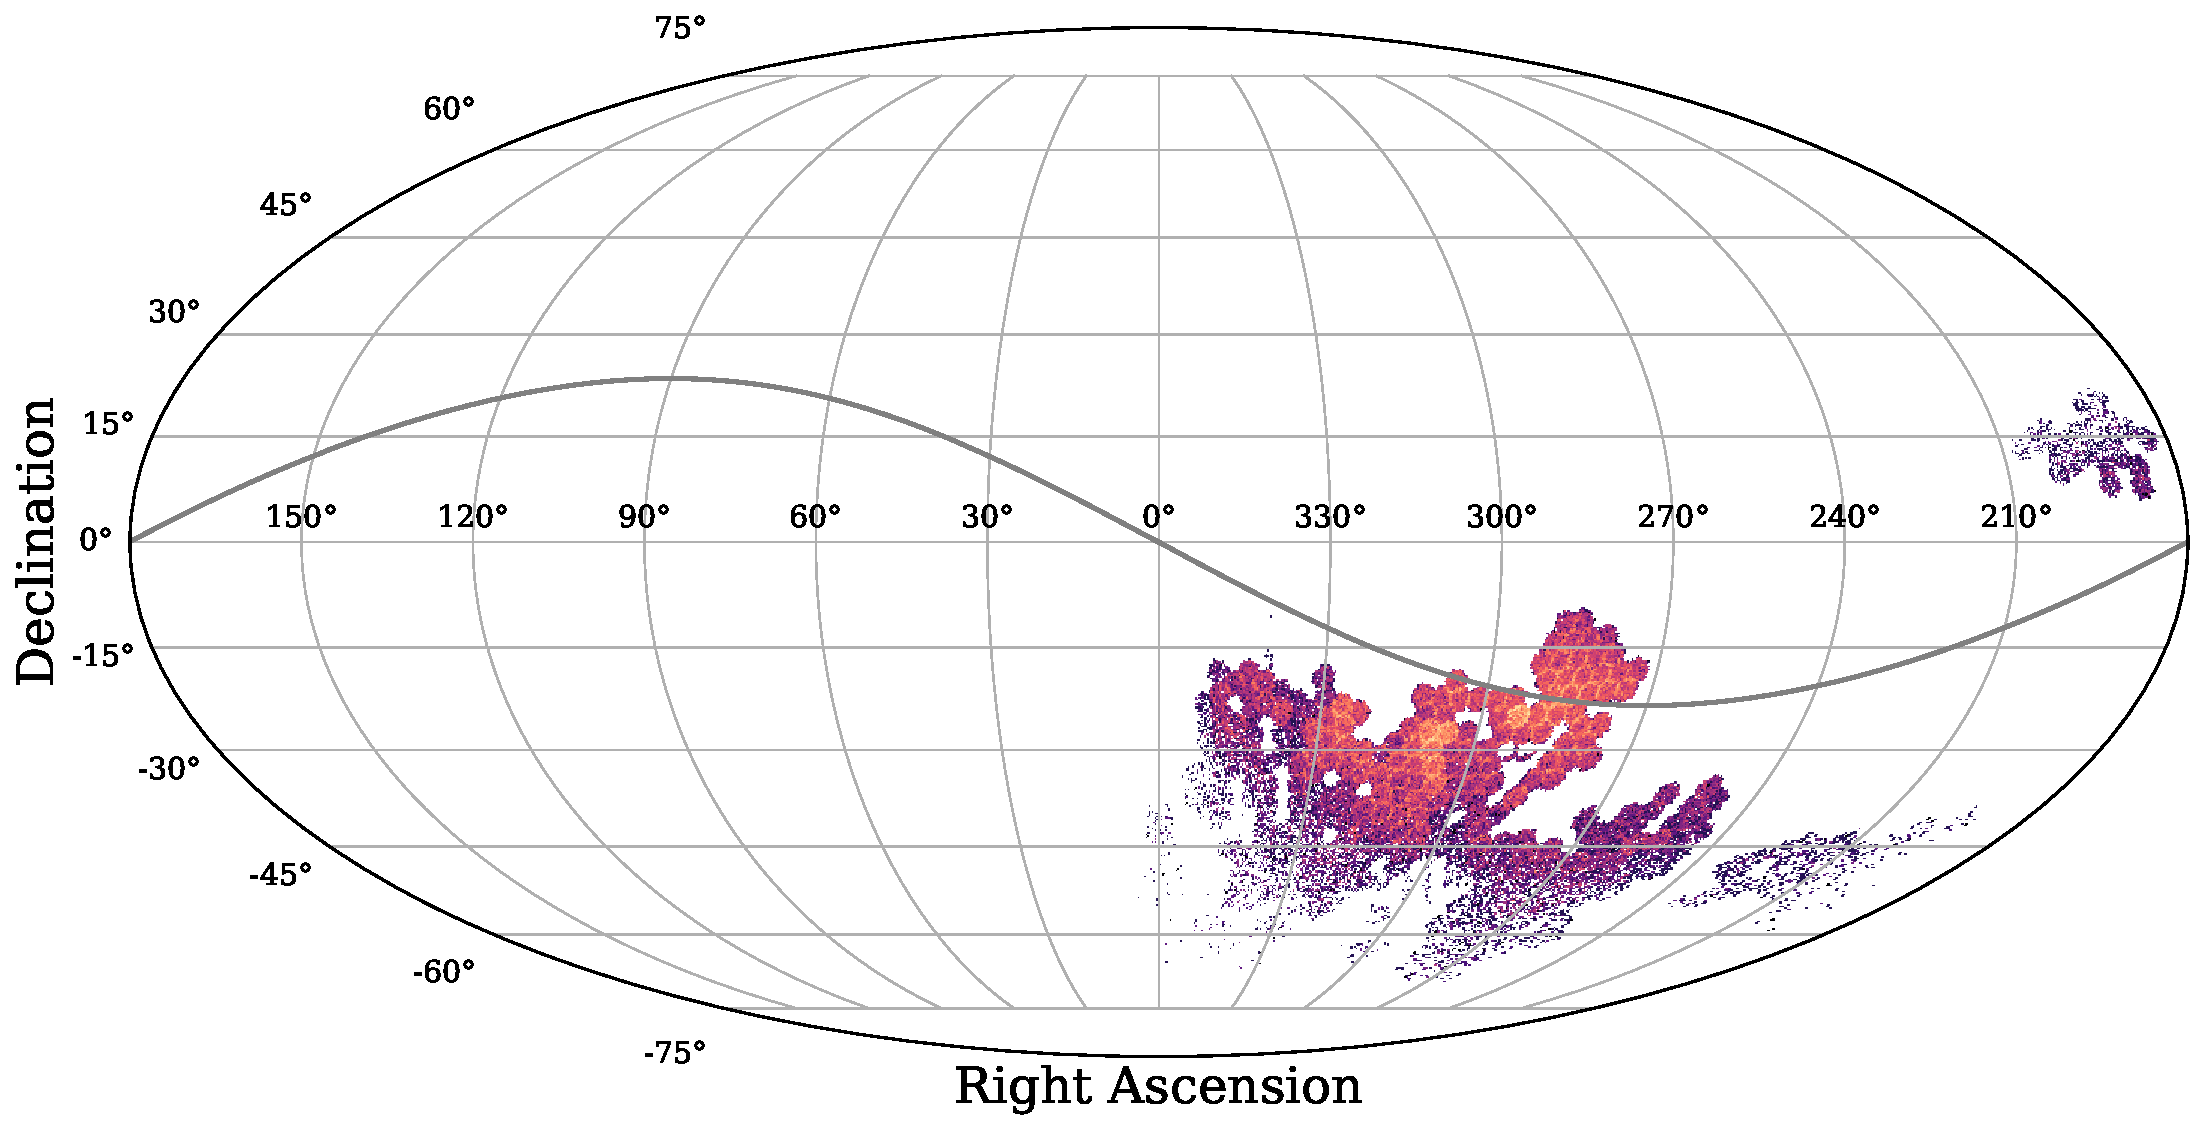
\includegraphics[width=\columnwidth]{observations_example.pdf}
    \caption{An example of asteroids detected in a single night of LSST observations. This example has ${\sim}420,000$ observed asteroids, of which ${\sim}1000$ are NEOs. Brightness of points indicates the number of asteroids in the pixel. Grey curve indicates the ecliptic plane.}
    \label{fig:observations_per_night}
\end{figure}

\subsection{Building and Scoring Tracklets}\label{sec:digest2_score}
Many NEOs will be instantly recognised as such from their angular velocities, since an object moving faster than 1.5 degrees per day will leave trails of 1.25 arcseconds in a 30s LSST exposure. We find that approximately 10\% of NEOs observed by LSST surpass this threshold, whilst no MBA is observed moving beyond this velocity. We predict that, on average, each night we will observe 21 trailed NEOs, which would then be submitted to the NEOCP. We remove these sources from our analysis and discuss them in Section~\ref{sec:trailed_neos}, since ambiguity between NEOs and MBAs is only a problem for the slower-moving NEOs. Herein, we probe ways to remove this remaining ambiguity.

We begin our analysis by selecting observations from the simulated LSST dataset that correspond to tracklets. For a tracklet to be built, we require it to satisfy the following criteria:
\begin{enumerate}
    \item \textbf{Number of observations:} We consider only objects which have at least 3 observations on a given night (we also consider more stringent criteria of 4+ observations - see Section~\ref{sec:traffic_basic}).
    \item \textbf{Maximum time separation:} We set the maximum time between observations to 90 minutes. Thus we only allow tracklets that have at least one pair of observations that occur within 90 minutes.
    \item \textbf{Minimum arc length:} We ensure that each tracklet is at least 1 arcsecond in length (corresponding to ${\sim}5$ pixels on Rubin's LSSTCam camera). This ensures that the motion vector of the tracklet can be determined.
\end{enumerate}
The motivation behind these cuts is to ensure that the tracklet constrains the on-sky motion of the object sufficiently well, so that its position at a later time can be easily extrapolated. With fewer observations or shorter tracklets, many different orbits could reproduce the same motion on the sky. Moreover, observations that are separated too significantly in time may be spurious linkages, where observations of multiple objects are incorrectly assumed to be of the same source.

A single tracklet in itself doesn't determine the orbit. Tracklets do place constraints on the direction and rate of motion which can be used -- when compared to the known populations of objects -- to determine the probability of the object having a particular orbit. These can then be marginalized over classes of interest to score the chance of an object belonging to any given class of objects. The main criterion the Minor Planet Center uses to place an object on the NEOCP is an NEO \dig{} score of at least 65. This score, ranging from 0 to 100, quantifies the probability that the object is an NEO and is calculated using the eponymous \dig{} code \citep{Keys+2019}.

\begin{figure}[htb]
    \centering
    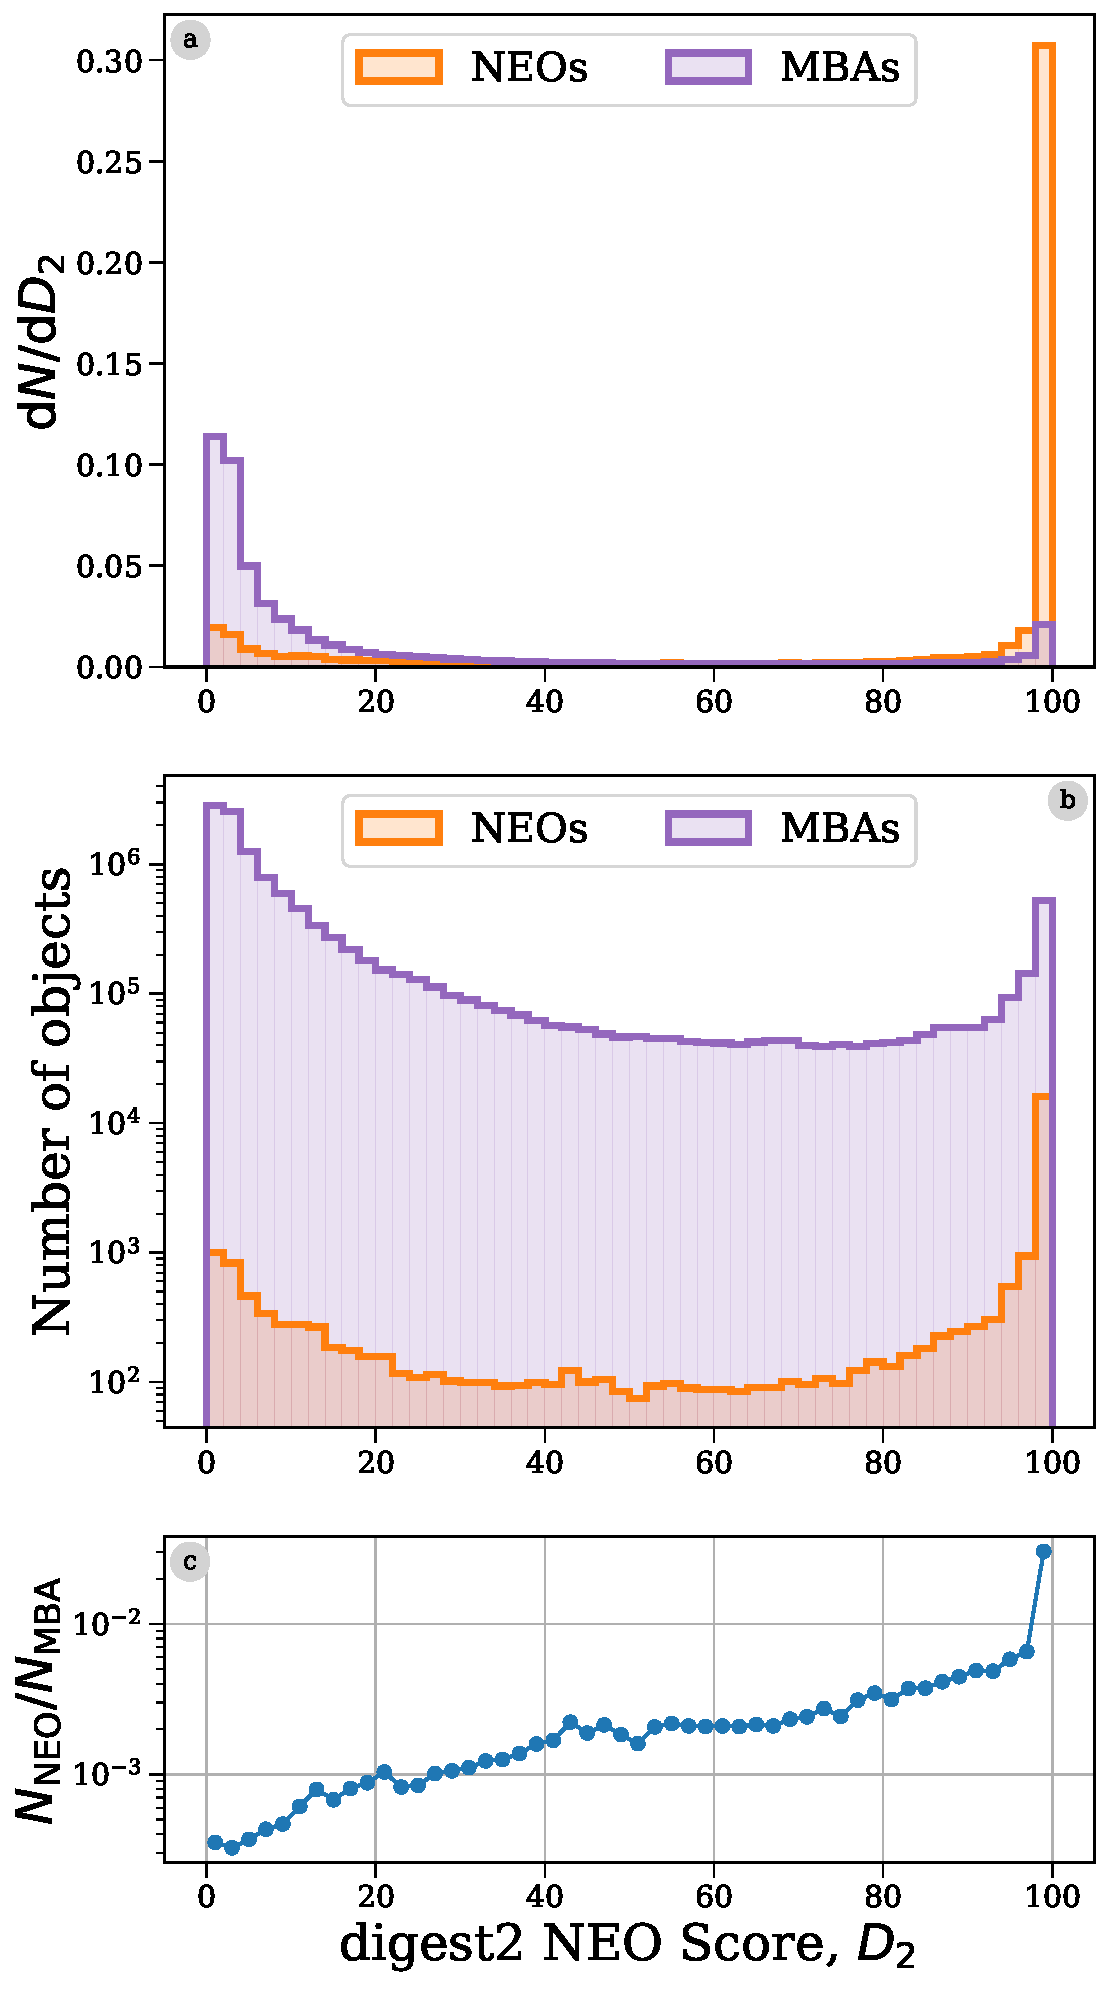
\includegraphics[width=\columnwidth]{digest2_pollution.pdf}
    \caption{The \dig{} score cannot adequately distinguish NEOs in the presence of a large MBA background. \dig{} scores for all NEOs and MBAs observed in the first year of our simulated LSST observations. \textbf{(a)} normalised histograms of \dig{} scores, \textbf{(b)} the same histograms un-normalised \textbf{(c)} ratio of the histograms in (b). Note that the latter two panels are on a logarithmic scale.}
    \label{fig:digest2_example}
\end{figure}

At its core, \dig{} compares a simulated catalogue of solar system objects to observed tracklets to estimate the probability that an object is an NEO. \dig{} bins simulated objects into 15 different orbit classes, using bins of perihelion, eccentricity, inclination and absolute magnitude. Then, for each observed tracklet, \dig{} samples a series of possible distances and radial velocities and uses those values to estimate possible orbits of the object. These orbits are binned and assigned a class based on the bin they are assigned. The NEO score is then estimated as a fraction of the orbits that are classified as NEOs. For a more exhaustive description of \dig{}, see \citet{Keys+2019}. We use \dig{} to calculate the NEO score of each tracklet in our sample. 
\begin{figure*}[htb]
    \centering
    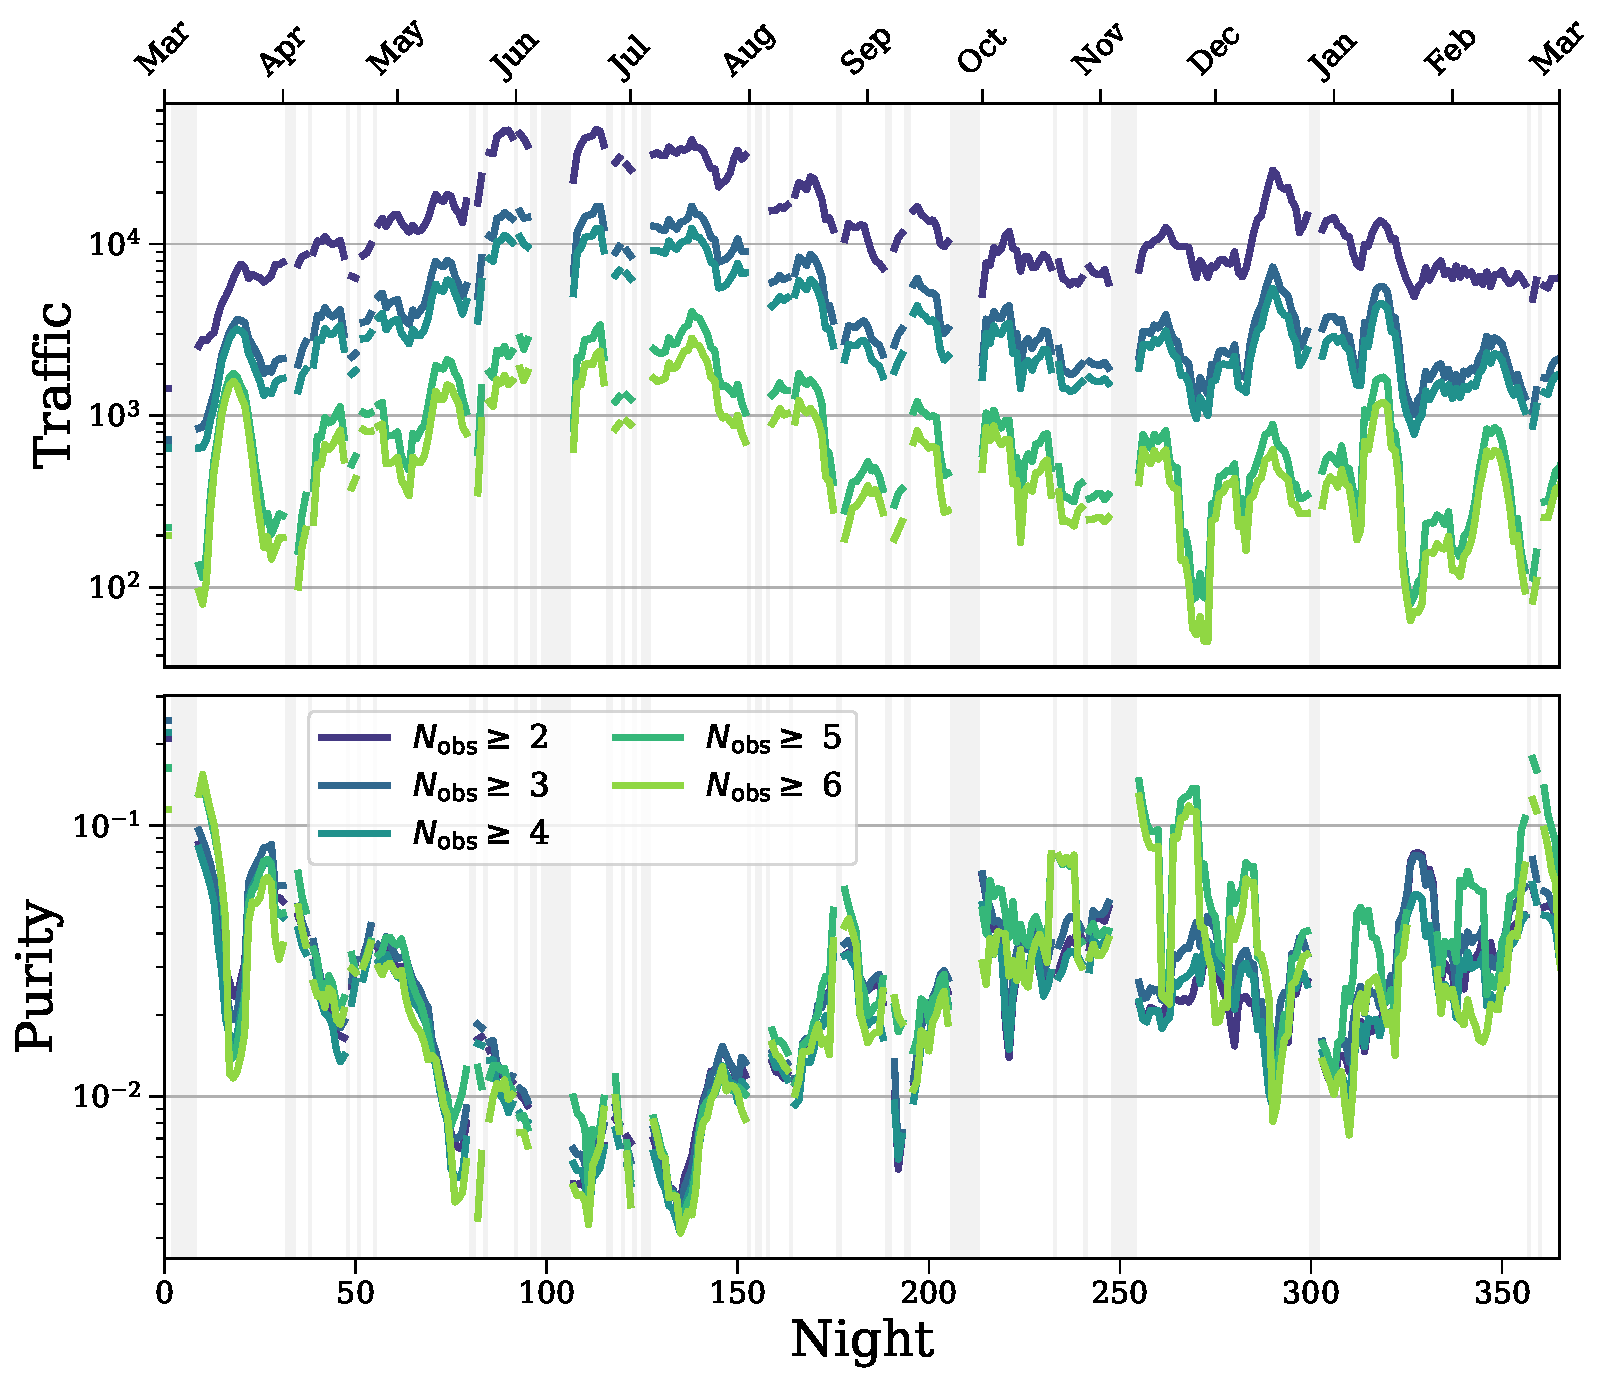
\includegraphics[width=\textwidth]{traffic_purity.pdf}
    \caption{The NEOCP would be overwhelmed by LSST submissions with current submission criteria. Traffic (number of objects sent) and purity (fraction of objects sent that are NEOs) of the NEOCP during the first year of LSST if every observation that qualifies for submission and with an apparent magnitude of $m < 22$ is submitted. Each line is plotted using a rolling window of 10 days to smooth stochastic effects. Different colours correspond to different constraints on the number of observations for a tracklet to be submitted. The dashed $N_{\rm obs} > 3$ line indicates the submissions of any magnitude (not limited to $m < 22$). Nights on which no observations were taken are highlighted with grey areas.}
    \label{fig:neocp_traffic}
\end{figure*}

The distribution of \dig{} scores for the NEOs and MBAs in the first year of observations is shown in Figure~\ref{fig:digest2_example}. As one would expect most NEOs have scores around 100, whilst most MBAs have scores around 0. However, we can already see that due to the sheer volume of MBA observations, the \dig{} score alone will not will not result in a high-purity sample of NEOs candidates. In particular, an object assigned a score of 65 or more only has a 1.4\% chance of actually being an NEO. Even with a score of 100 the probability is still only 8.6\% (Figure~\ref{fig:digest2_example}c). We discuss this further in Section~\ref{sec:discussion}.

Additionally, since many objects observed by LSST will be too faint for external follow-up, we consider apparent magnitude as an additional criterion for submission to the NEOCP. The MPC observation archive\footnote{\url{https://minorplanetcenter.net/iau/ECS/MPCAT-OBS/MPCAT-OBS.html}} includes the magnitude of each observation at discovery. We cross-referenced this with the list of known NEOs and find that the 98th percentile in apparent V-band magnitude, $m$, is 21.73. We therefore apply a conservative threshold of $m < 22$ for an object to be submitted to the NEOCP to ensure that external follow-up is possible for each object.

\subsection{Traffic and Purity of NEOCP}\label{sec:traffic_basic}

\begin{figure*}
    \centering
    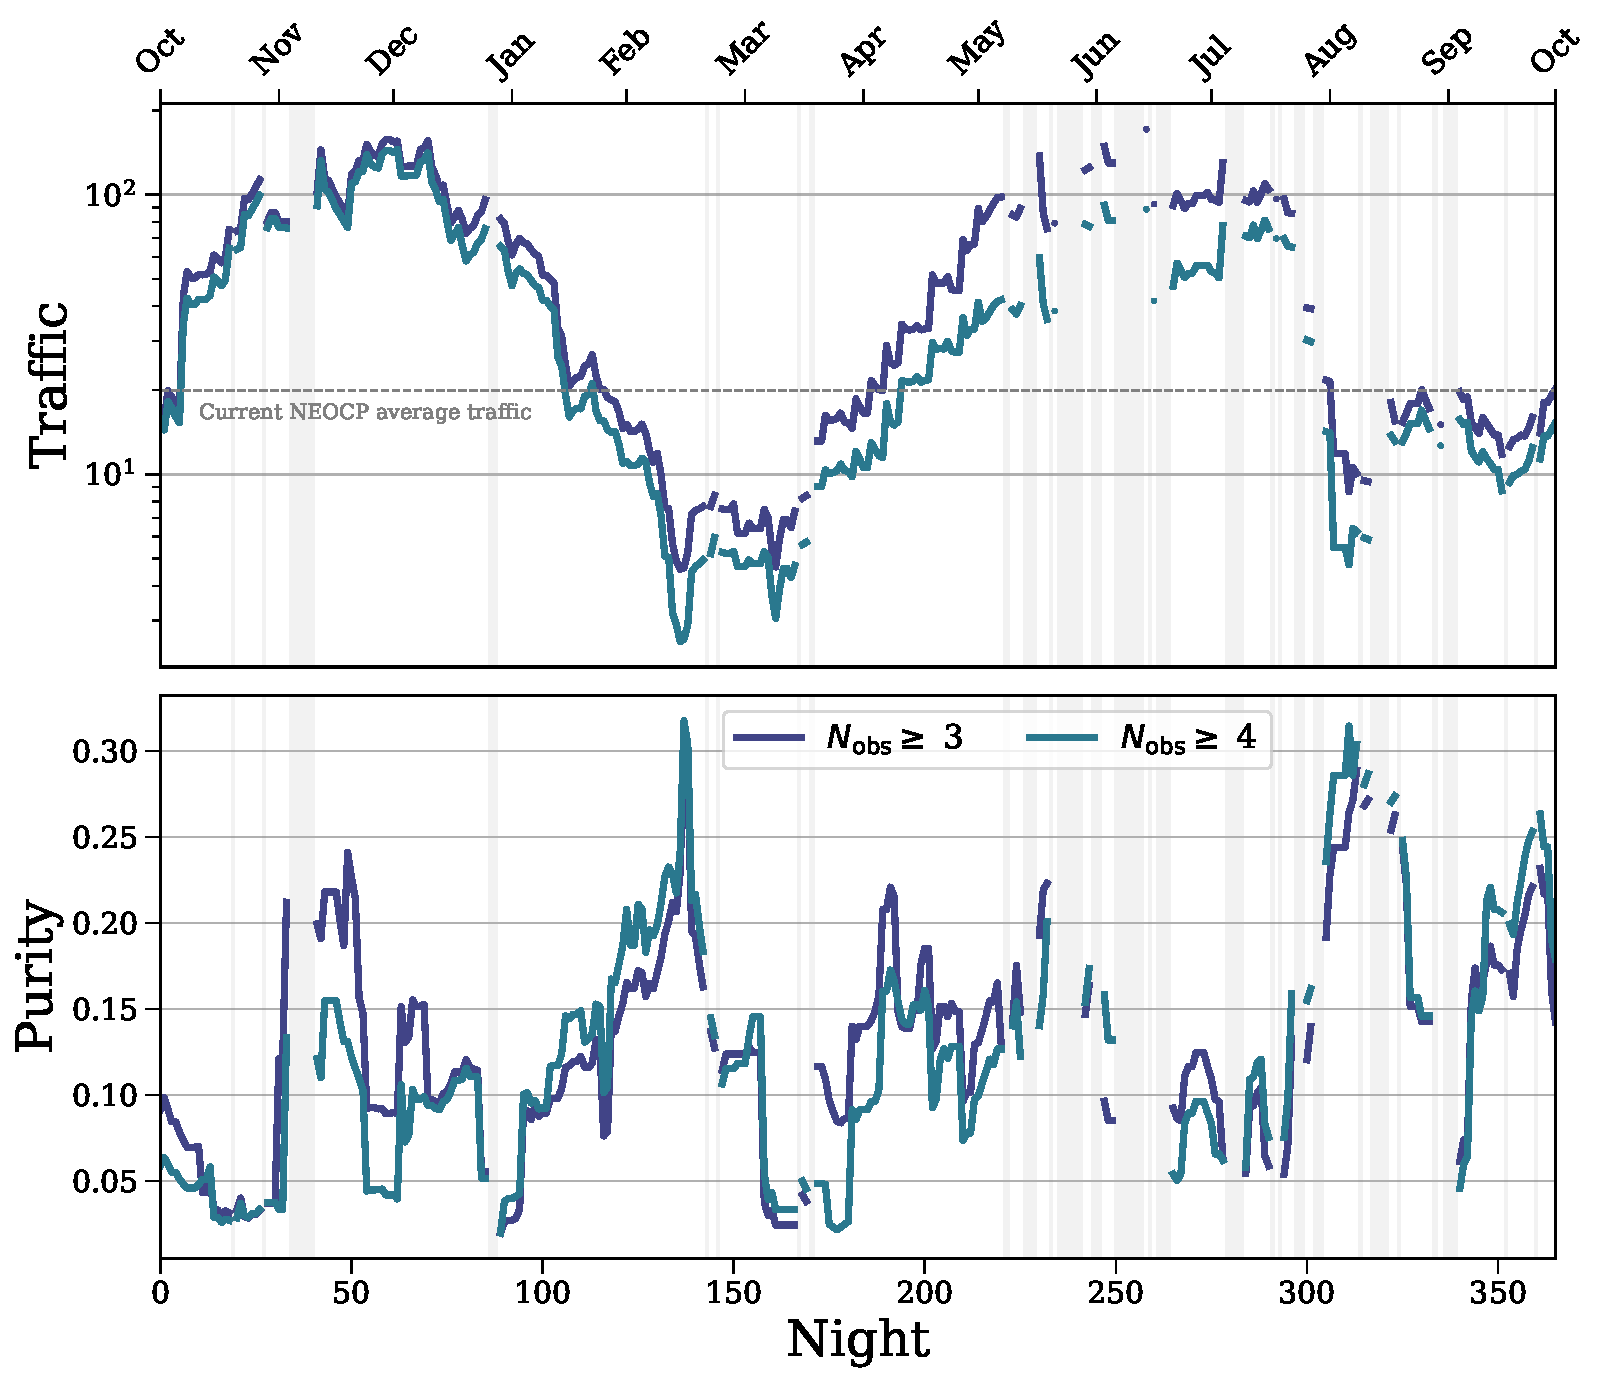
\includegraphics[width=\textwidth]{traffic_purity_unfindable.pdf}
    \caption{NEOCP submissions would remain at reasonable levels if we knew a priori which objects LSST would self-follow-up. As Figure~\ref{fig:neocp_traffic}, but only including objects that would not be detected by LSST alone. Note the y-scale of the lower panel is linear.}
    \label{fig:neocp_traffic_unfindable}
\end{figure*}

In Figure~\ref{fig:neocp_traffic}, we summarise the effect that LSST submissions would have on the NEOCP if \textit{every} tracklet that met the \dig{}~$>65$ and $m < 22$ cut were submitted. The top panel shows the traffic of the NEOCP, meaning the number of objects that would be submitted to the page, whilst the bottom panel shows the purity, meaning the fraction of objects submitted to the page that are actually NEOs.

The current typical traffic of the NEOCP is on the order of two dozen new submissions per night. This would increase by 2 orders of magnitude as a result of LSST submissions. Each line corresponding to a different number of minimum nightly observations (each increasing from the original choice of 3 as discussed in Section~\ref{sec:digest2_score}). Although the traffic is lower when requiring more observations, even when requiring a minimum of 6 observations the traffic can still reach several hundreds of submissions per night, and at low purity. This is more than the follow-up system is currently set-up to handle.

The purity of the NEOCP is also severely impacted by Rubin observations, with the abundant MBA observations contaminating the sample. For almost the entire the candidates would have a purity below 10\%, with dips to as low as 0.2\%. As noted in Section~\ref{sec:digest2_score}, this is due to the sheer abundance of \emph{uncatalogued} MBAs in Rubin observations. Therefore, given these purity levels, a significant amount of follow-up time would be spent re-observing MBAs masquerading as NEOs.

There is a clear seasonal variation over the year as the ecliptic plane moves through the sky. Rubin observes from the southern hemisphere and thus around July when the ecliptic is at lower declinations, more MBAs will be observed. This both increases the traffic and decreases the purity of the NEOCP.

Overall it is clear that, if we proceed in the same manner as is currently recommended, the NEO follow-up community will not be able to handle the load.

\subsection{The best-case scenario: The NEOCP without tracklets Rubin will follow-up on its own}\label{sec:no_LSST_detections}

Given it repeatedly re-observes large swaths of the sky, Rubin can follow-up many potential NEOs on its own, providing sufficient astrometry for accurate orbit determination without external contributions. If we perfectly knew which objects would be followed up by Rubin itself, this would dramatically reduce the number of tracklets listed on the NEOCP -- and allow the community to focus on ones that truly \emph{require} follow-up in order to be designated.

Rubin requires the pipelines link 95\% of objects observed on at least 3 separate nights within a 15 day window, each with at least 2 observations separated by at most 90 minutes \citep{oss}. As these pipelines are still under development, we compute how many objects Rubin can link on its own by using a python package \texttt{difi} \citep{difi}. This package emulates a ``perfect linker'', identifying tracklets that Rubin pipelines will be able to link and compute orbits for. We've confirmed that the development version of Rubin linking pipelines are very close to the performance emulated by \texttt{difi} (Ari Heinze, priv. comm.).

In Figure~\ref{fig:neocp_traffic_unfindable}, we reproduce an analogue of Figure~\ref{fig:neocp_traffic}, but now only including objects that would \emph{not} be detected by LSST alone. This represents a best case scenario in which we had foreknowledge of which observed objects would be detected. In this scenario we see that the traffic from LSST rarely exceeds more than 100 objects and is often only a handful. Similarly the purity is much higher, with an average of around 14\%. We conclude that if we were to know whether an object would be detected by LSST, the load on the NEOCP would remain at manageable levels. Motivated by this result, we next look at developing an algorithm that predicts whether an object can be detected by LSST alone.

\section{Mitigating the impact of LSST}\label{sec:mitigation}

\subsection{Estimating the Probability of self-follow-up}\label{sec:pred_alg}
As illustrated in Section~\ref{sec:no_LSST_detections}, if we were able to tell ahead of time which NEO candidates the LSST will be able to link on its own, we could remove or de-prioritise them on the NEOCP. While this is in principle impossible -- LSST's schedule is dynamic, the weather cannot be predicted, and the NEO candidate itself could take many different paths on the sky -- we \emph{can} estimate the \emph{probability} that of self-follow-up.

The technique is conceptually simple. Given a single tracklet, it's straightforward to compute the ensemble of ranges and radial velocities $(D, \dot{D})$ of NEOs consistent with that tracklet. Secondly, we can compute the expected series of Rubin observations for the next month, assuming clear weather. Finally, we cross-correlate the two, and compute the fraction of the NEO ensemble that would be recovered.

The details and the implementation are as follows. In order to determine the location of an object on subsequent nights one needs to estimate its orbit. Each object on a given night consists of at least two observations, $O$, that have the form
\begin{equation}
    O = \{ \alpha, \delta, t \}
\end{equation}
where $\alpha$ is the right ascension, $\delta$ is the declination and $t$ is the time of observation. We determine the proper motion of the object on the sky, ($\dot{\alpha}$, $\dot{\delta}$), by calculating the change in position between the two observations using \texttt{Astropy SkyCoord} and dividing by the time between observations. This determines 4 of the 6 orbital elements, but the topocentric distance, $D$, and radial velocity, $\dot{D}$, of the object are unconstrained.

We draw a sample of $D$ uniformly in log-space between $[0.1, 10] \unit{au}$ and a sample of $\dot{D}$ uniformly between $[-50, 10] \unit{km}{s^{-1}}$ to create a grid of $(D, \dot{D})$. Combining these with the measured $(\alpha, \delta, \dot{\alpha}, \dot{\delta})$ values (and adding $0.1^{\prime\prime}$ of scatter to the measured on-sky positions to account for the detector uncertainty), we create a series of possible variant orbits for the object. We use the functionality in the \texttt{THOR} package \citep{Moeyens+2021} to handle the orbital dynamics and celestial mechanics (including light-time travel corrections). Since we are only interested in NEOs, we mask out any orbits that have a perihelion distance of greater than $1.3 \unit{au}$. To demonstrate the different possible orbits that we could infer from a single observation, we plot a subset of the variant orbits obtained for an NEO observed in our mock observations in Figure~\ref{fig:orbits}.

\begin{figure}[htb]
    \centering
    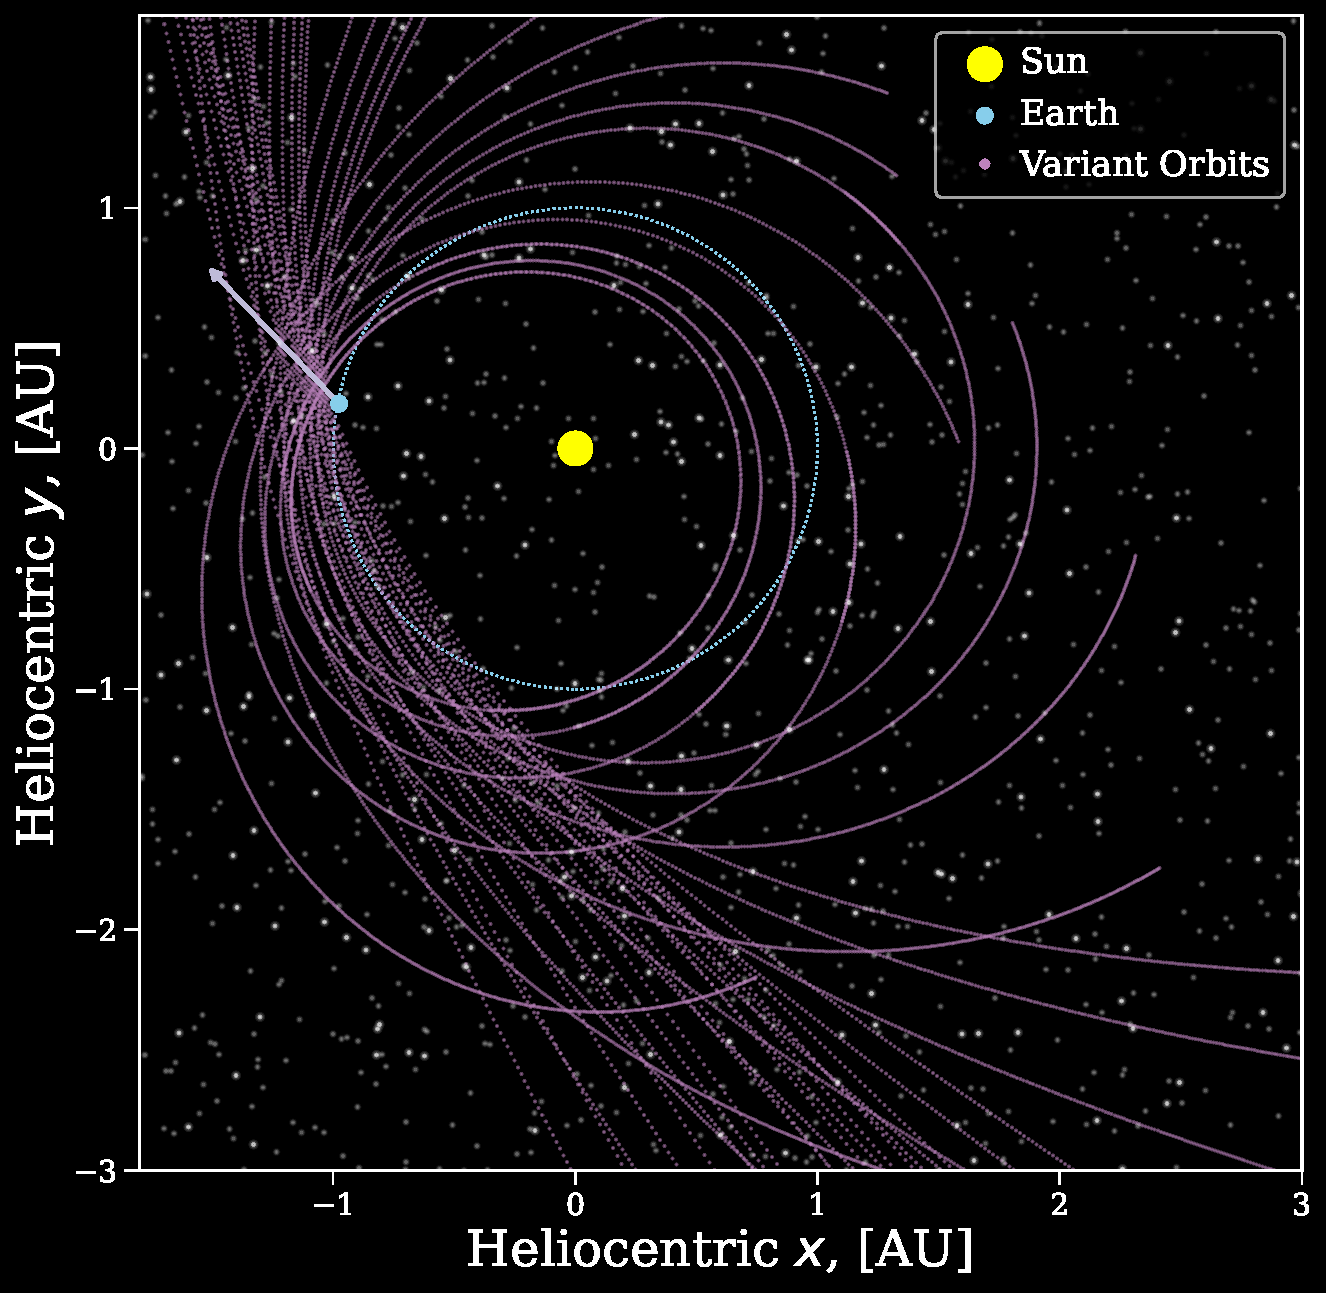
\includegraphics[width=\columnwidth]{figures/orbits_example_small.pdf}
    \caption{Variant orbits computed for an example NEO in our sample based on a single night of mock LSST observations. The white arrow indicates the initial sight-line for the observation. The blue dotted line indicates the orbit of the Earth. Background stars are for illustrative purposes only.}
    \label{fig:orbits}
\end{figure}

% \begin{figure}[htb]
%     \centering
%     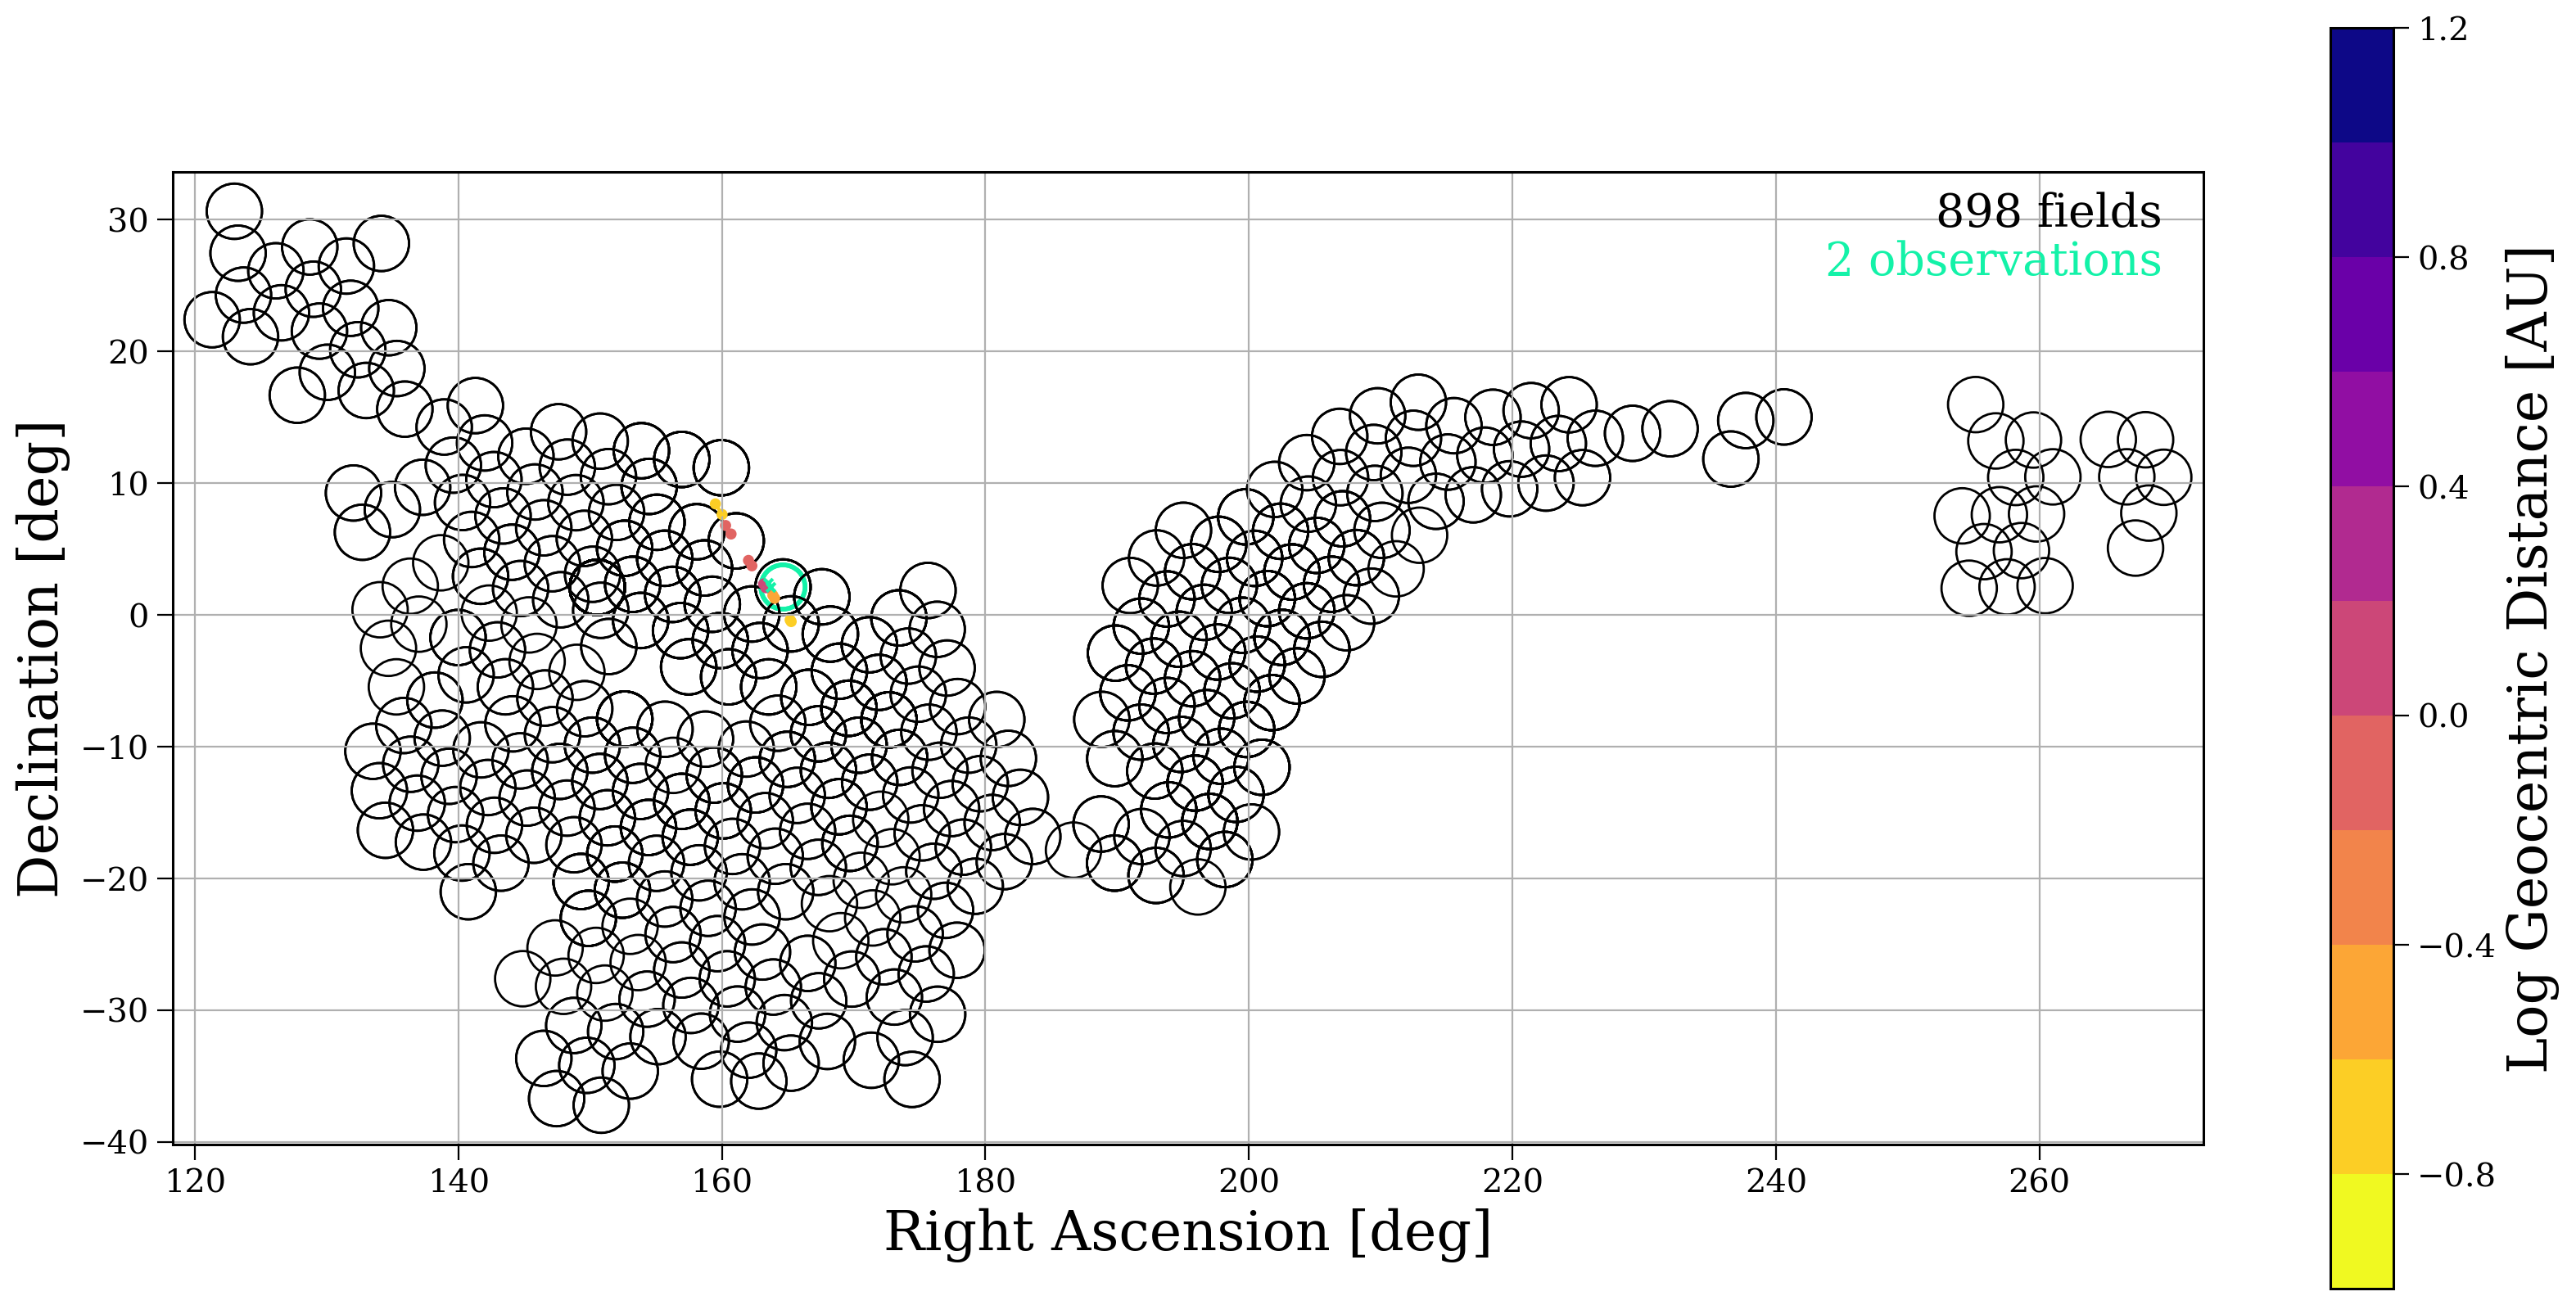
\includegraphics[width=\columnwidth]{methods_placeholder.png}
%     \caption{A demonstration of the LSST detection probability prediction. Black circles (to scale with $2.1^{\circ}$ radii) represent a bounding circle of LSST's camera footprint for each visit in this night's predicted schedule. For each orbit we plot the object's predicted location at the start and end of the night and colour them by the assumed distance. In cyan we show true position of the object and outline any visits that produce an observation in cyan also.}
%     \label{fig:circles}
% \end{figure}

Additionally, we estimate the absolute magnitude of the object for each orbit using the $HG$-system \citep{mpc_h_g}. This is needed to assess whether the object will be bright enough to detect in subsequent observations. To convert to LSST band magnitudes, we assume a C-type asteroid and mean colours adopted from \citep{Jones+2018}. For the slope parameter, we assume the customary $G=0.15$ \citep{mpc_h_g}. The phase angle is also taken into account.

% We additionally calculate the phase angle of the asteroid, $\alpha$, as
% \begin{equation}
%     \cos \alpha = \frac{D_{a, \odot}^2 + D_{a, \oplus}^2 - D_{\odot, \oplus}^2}{2 D_{a, \odot}^2 D_{a, \oplus}^2}
% \end{equation}
% where $D_{a, \odot}$ is the distance between the asteroid and the Sun, $D_{a, \oplus}$ is the distance between the asteroid and the Earth and $D_{\odot, \oplus}$ is the distance from the Sun to the Earth. We then use the mean observed V-band magnitude, the assumed distances, the phase angle and a fixed slope parameter of $G = 0.15$ (as is customary) to calculate the current absolute magnitude \citep{mpc_h_g}.

For each night in the first year, we use \texttt{rubin\_sim} to create a predicted schedule for the following 14 nights, our assumed detection window \citep{rubin_sim}. These predicted schedules represent an estimate of where LSST will look next and as such account for scheduled downtime, but do not include unscheduled downtime or poor weather conditions. This means our predicted schedule represents the best-case scenario; once Rubin is in commissioning and additional information about the weather becomes available it will be straightforward to incorporate it into the analysis.

Next, using \texttt{OpenOrb}, we produce ephemerides for all variant orbits at times of each visit in the following 14 nights of the predicted schedule \citep{Granvik+2009}. For each orbit and each visit, we check whether the object is within the LSST camera footprint, and whether it's bright enough to be detected using Rubin's canonical $5\sigma$ cutoff. If both of these criteria are met then we assume an observation has been made.

\begin{figure*}[htb]
    \centering
    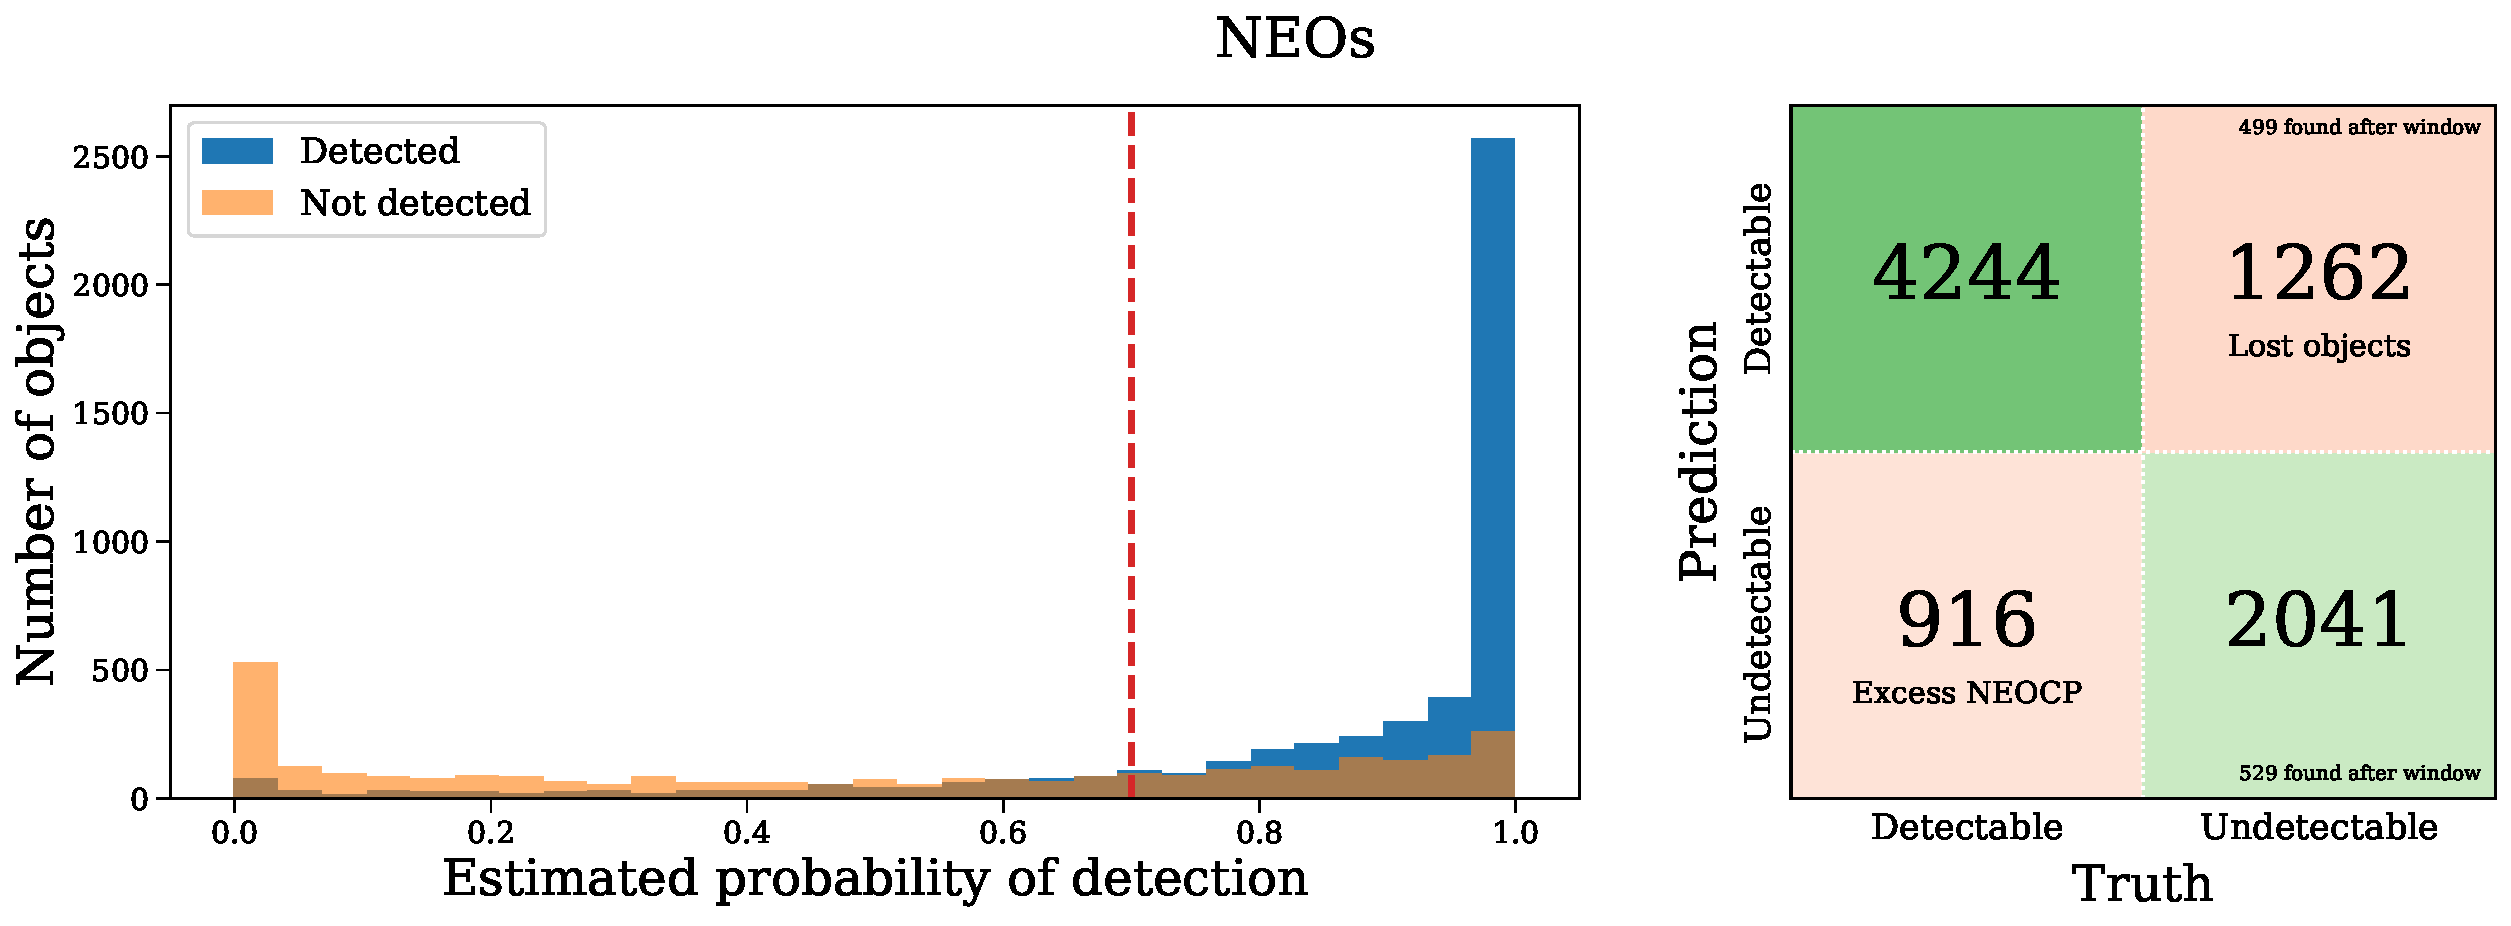
\includegraphics[width=\textwidth]{contingency_neo.pdf}
    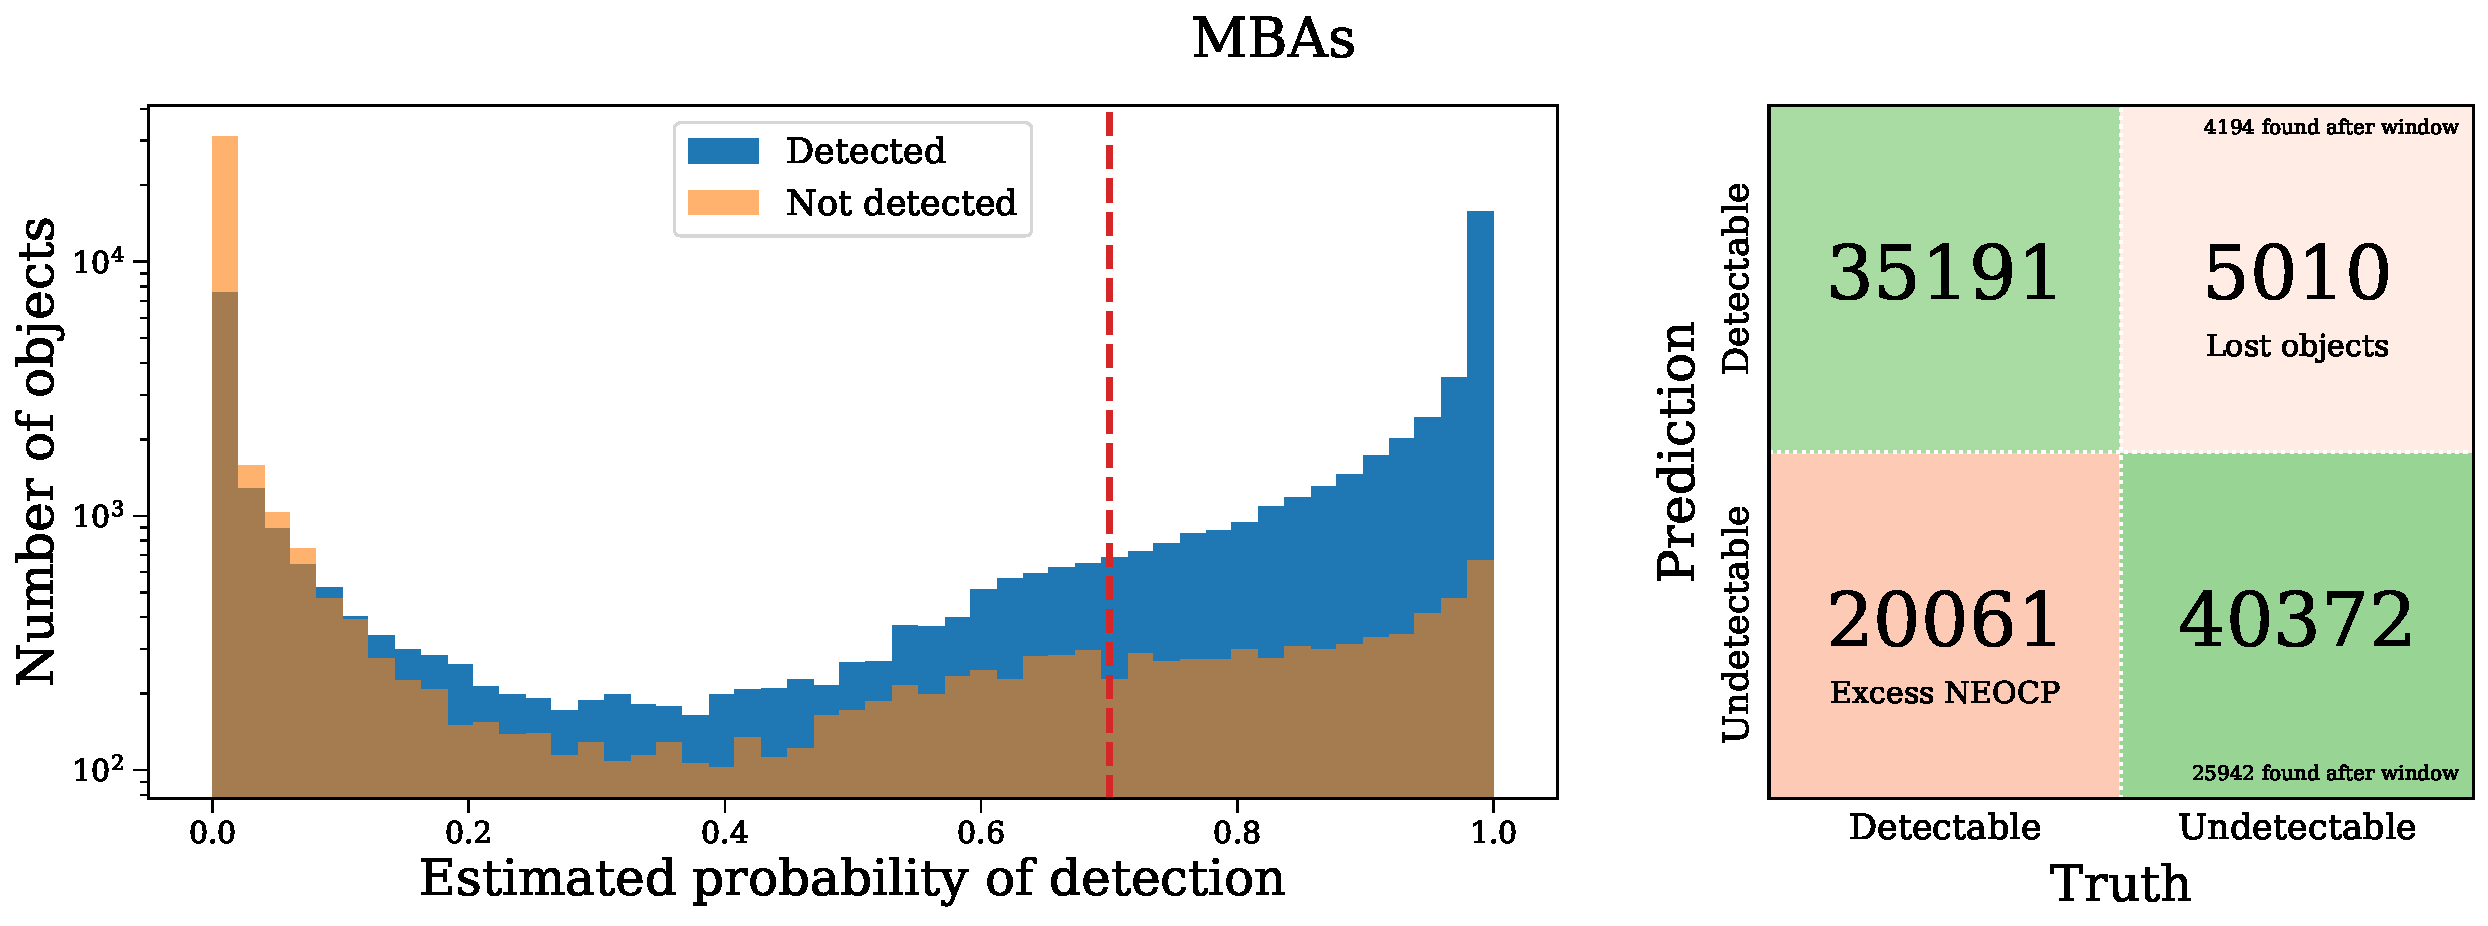
\includegraphics[width=\textwidth]{contingency_mba.pdf}
    \caption{A demonstration of the prediction algorithm described in Section~\ref{sec:pred_alg} using 1 year of simulated observations for both NEOs (top) and MBAs (bottom). \textbf{Left:} Probability that an object will be detected within 15 nights, split into a population of objects that are \textit{actually} detected within 15 nights in the simulated observations and a population that are not. The red dashed line indicates our threshold of $\thresholdAlg{}$ for submission to the NEOCP. Note that the histogram is on a logarithmic scale for the MBAs. \textbf{Right:} A contingency matrix representing the algorithm's ability to predict the detectability of an object.}
    \label{fig:contingency}
\end{figure*}

Finally, we identify variant orbits whose tracklets satisfy LSST linking requirements: have at least 2 observations on at least 3 nights in a 15 day window, with each having a minimum arc length of 1 arcsecond and maximum time separation of not more than 90 minutes \citep{oss}. We also account for prior observations in this calculation. For example, when assessing the probability of linking of an object that observed on (say) night 10, we take into account that that object has previously been observed on (say) night 8, and so even a single additional future tracklet in the linking window (on, say, night 14) is sufficient for linkage. Following this procedure, the overall probability of the object being detected by LSST then a simple ration of linked to all variant orbits.

\subsection{Mitigation by avoiding follow-up of likely-to-be-linked objects}\label{sec:using_alg}
We now examine the effect of applying the LSST detection probability algorithm to reduce the load on the NEOCP. Figure~\ref{fig:contingency} shows the results for a year of simulated observations for both the NEOs and MBAs, including only objects that we would potentially submit to the MPC (at least 3 observations in the initial tracklet and with an apparent magnitude of at most $22$). The histograms show the estimated probability of detection by LSST for each object, split into a population of objects that are \textit{actually} detected within 15 nights in our simulated observations and a population that are not. On average the algorithm predicts the correct outcome approximately $\efficiencyAlg{}\%$ of the time.

We use a threshold of $\thresholdAlg{}$ for deciding whether an object will be detected by LSST. We found that this value was ideal for minimising the number of NEOs that are lost and the number of objects sent to the NEOCP, whilst maximising the fraction of those objects that are NEOs.

In the right side of Figure~\ref{fig:contingency}, we show contingency matrices for both NEOs and MBAs when applying this threshold. The lower left quadrants give a count of the number of objects that will be sent to the NEOCP needlessly as LSST will detect them without follow-up. The upper right quadrants total the number of objects that will be lost, since LSST will not detect them within the given detection window but they would also not be sent to the NEOCP. We additionally annotate the number of objects that would be found after the detection window and note this reduces the overall number of lost objects.

Overall, when applying this threshold, we find that, on average, $\npernightAlg{}$ objects would be submitted to the NEOCP per night, but only around $\purityAlg{}\%$ (${\sim}\purityAlgRaw{}$) of those objects would be NEOs. Moreover, $\neoLostAlg{}$ NEOs would remain undetected by LSST and not be sent to the NEOCP for follow-up. This method would reduce the traffic on the NEOCP by more than an order of magnitude, however there is only a small improvement on the purity of the submitted objects and the vast majority of submissions would still be MBAs. 

\section{Discussion} \label{sec:discussion}
As we have shown above, even when applying our LSST detection probability algorithm, the NEO follow-up community would be overwhelmed by submissions from LSST and significantly more MBAs would be submitted than NEOs. In this section we consider recommendations for how to lessen these issues and ensure that the NEOCP remains functional in the era of LSST.

\subsection{Improve the \dig{} algorithm}
In Figure~\ref{fig:digest2_example} we highlighted that \dig{} struggles to distinguish between NEOs and MBAs when dealing with the extreme volumes of previously unknown MBAs that LSST will observe. When using the first year of simulated LSST observations, we find that only ${\sim}1.4\%$ of objects with a \dig{} NEO score of at least 65 (the threshold for submission to the NEOCP) are in fact NEOs.

For this reason, it is important to consider whether there are improvements that can be made to the \dig{} algorithm in distinguishing between NEOs and MBAs. Given the required suppression factor for MBAs and extensive prior work done on this algorithm, it is unlikely that such improvements would be able to eliminate this problem in all regimes. However, it is possible that there are still particular cases or particular areas of the sky in which the distinction would be improved. For instance, one could consider the following parameters:

\paragraph{Ecliptic Latitude} MBAs are constrained to reside within the asteroid belt and therefore close to the ecliptic. NEOs have no such restriction and hence observations with increased ecliptic latitudes are more likely to be NEOs (see Section~\ref{sec:ecl_lat}).

\paragraph{Apparent Magnitude} NEOs tend to be smaller in size than MBAs and therefore have fainter absolute magnitudes. In particular, we find that, for our sample, all MBAs have absolute magnitudes less than $H=23$, whilst NEOs extend up to $H=25$. However, in observations we instead measure the \textit{apparent} magnitude, for which the distinction is less clear cut. Yet we do still find that NEOs are in general concentrated more at fainter apparent magnitudes than MBAs. This criterion may be difficult to use in practice since it prioritising fainter objects for follow-up may be impractical.

\paragraph{Direction of motion on the sky} Since NEOs are much closer than MBAs, we would expect a much greater variation in direction of motion on the sky for NEOs. Specifically, it is unlikely for MBAs to be moving in a direction away from the ecliptic plane, whereas NEOs could be moving in almost any direction.

\paragraph{Rapid rotation} As mentioned above, NEOs are generally smaller than MBAs. This means that we would expect them to rotate faster given the same angular momentum. We can measure this rate as a variation in apparent magnitude and thus objects with a frequent variability in apparent magnitude may be more likely to be NEOs. In reality this may prove difficult since high photometric variability may also indicate a spurious linkage.\\

Each of these parameters alone may not be sufficient to isolate the NEO population - however one could consider them together and assign a probabilistic weight to each NEO score based on these parameters. A faint object may still be an MBA, but a faint, object detected at large ecliptic latitudes, moving away from the ecliptic plane is much more likely to be an NEO. In this way the \dig{} algorithm could take into account further observational data, rather than classifying entirely based on the orbit, to more effectively classify potential NEOs.

\subsection{Effect of the MBA background}
The main problem with NEO follow-up currently stems from the abundance of MBAs relative to NEOs. It is expected that after the first year of observations LSST will discover approximately $85\%$ of all MBAs down to its flux limit \citep{Juric+2020}. This will strongly suppress the number of MBAs that would be submitted to the NEOCP.

\begin{figure}[tb]
    \centering
    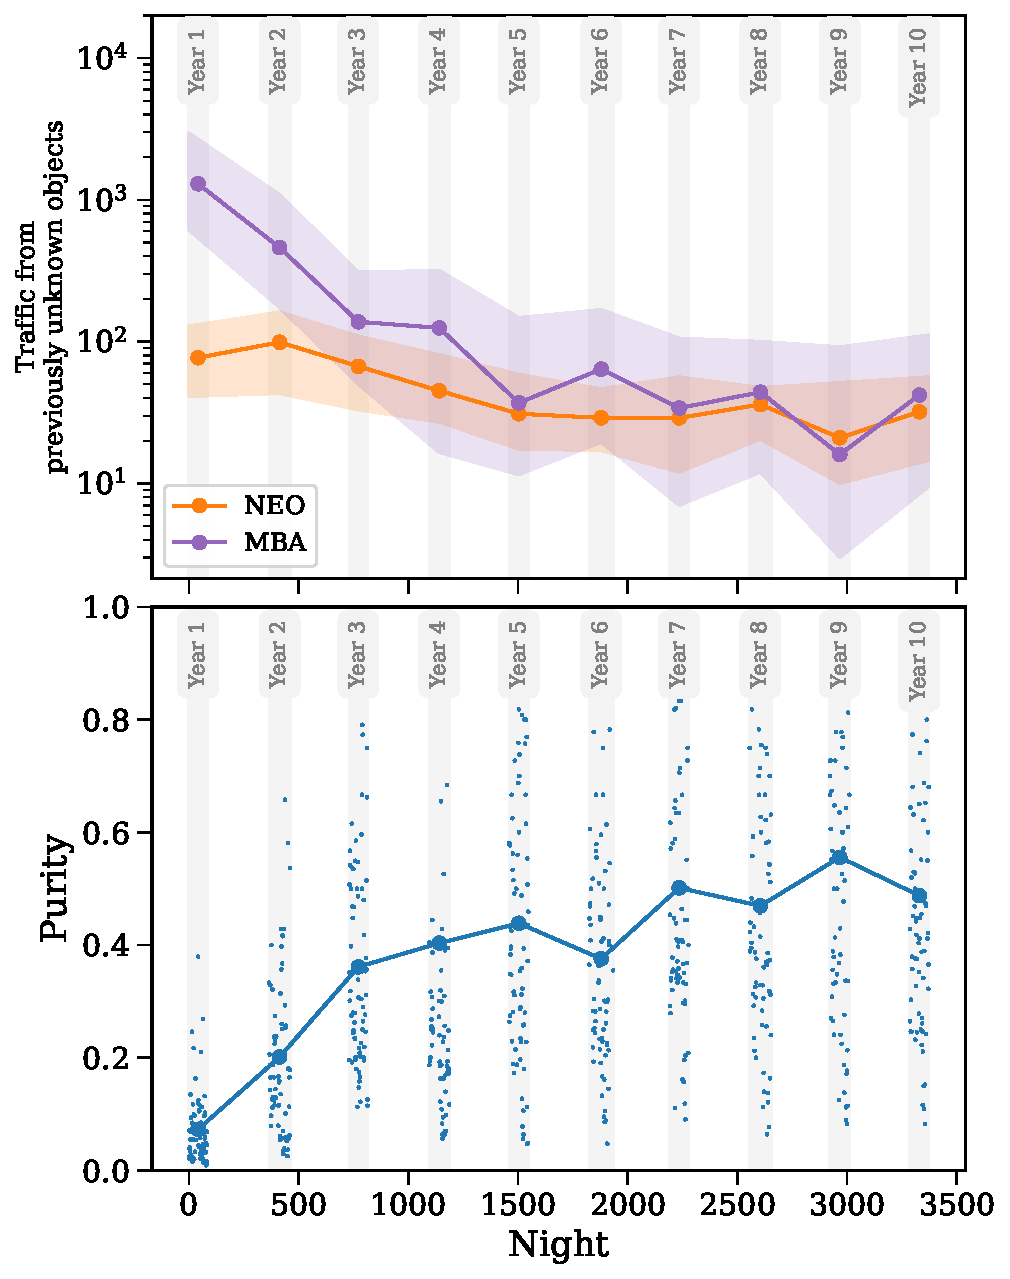
\includegraphics[width=\columnwidth]{figures/digest2_purity_over_lsst.pdf}
    \caption{\dig{} more accurately identifies NEOs once the previously unknown MBA population is catalogued. \textbf{Top:} Median number of previously undiscovered NEOs and MBAs with \dig{} scores $\ge 65$ over the first 75 nights without bad weather in each year. Shaded areas indicate interquartile range over those 75 nights. \textbf{Bottom:} Fraction of those objects that are NEOs averaged over the first 75 nights.}
    \label{fig:digest2_purity_improvements}
\end{figure}

At the same time, we expect a significant fraction of NEOs to be smaller objects that come for infrequent close approaches and so, even with new detections, we still expect a constant flux of new NEOs \citep{Juric+2020}. In this way the number of NEOs that are submitted to the page would remain roughly constant.

We demonstrate these trends in the top panel of Figure~\ref{fig:digest2_purity_improvements}. We show how the traffic from previously unknown objects in each population changes over the full 10 years of simulated observations (time at which objects become known calculated using \texttt{difi}, \citealp{difi}). For the NEOs we see that the gradient is roughly constant, meaning that a similar number of NEOs are detected on each night of the survey. However, for the MBAs, detections are skewed heavily towards the earlier years of the survey.

Therefore, once most of the MBAs have been identified, the traffic and purity of NEOCP submissions from LSST would be significantly improved. In the bottom panel of Figure~\ref{fig:digest2_purity_improvements} we show how the purity of submissions change over the survey. We can see that within 1-2 years, the purity reaches reasonable levels. Moreover, when applying our LSST detection probability algorithm in addition, we expect that the resulting traffic and purity would approximate the ideal case described in Section~\ref{sec:no_LSST_detections}.

The disadvantage of this approach of course is that one would need to wait until the first year of observations were complete. This means that any NEOs that will not be re-observed after the first year would not be sent for follow-up and may be lost. A potential solution to this problem is to apply a stringent ecliptic latitude cut in the first year and gradually relax it as MBAs are identified.

\subsection{Stringent Ecliptic Latitude Cut}\label{sec:ecl_lat}
Given that MBAs are constrained to lie within the ecliptic plane, ecliptic latitude, $b$, is a strong distinguishing factor between NEOs and MBAs. Since \dig{} will not effectively discriminate between NEOs and MBAs in the first year of LSST, one could instead apply a simple ecliptic latitude cut such that a minimum $\abs{b}$ is required.

\begin{figure}[tb]
    \centering
    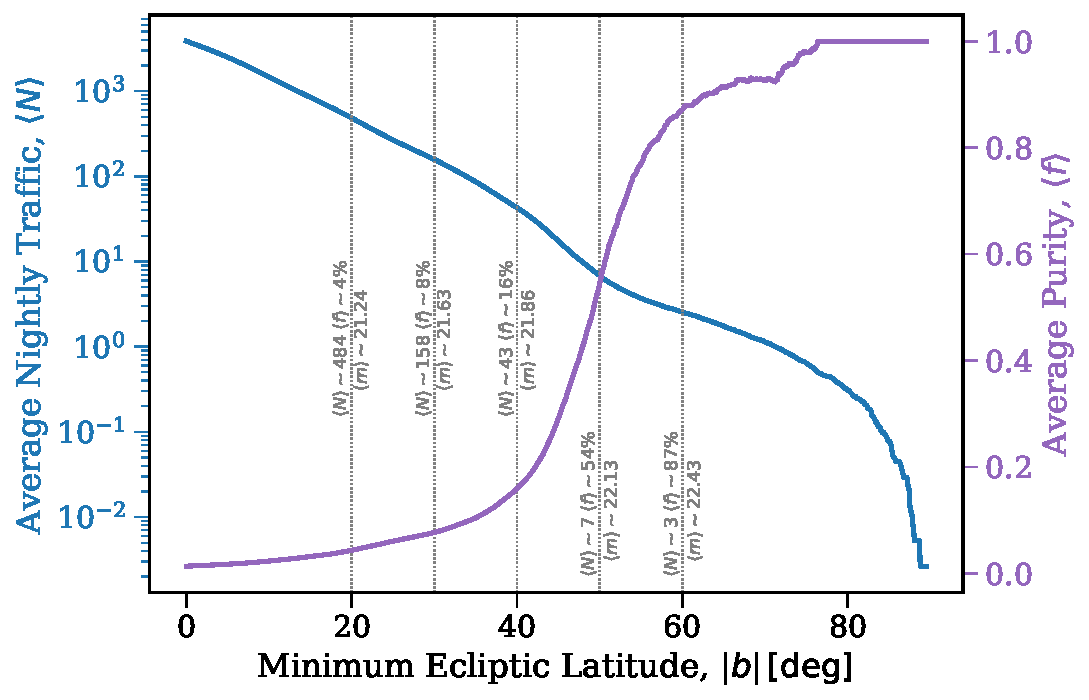
\includegraphics[width=\columnwidth]{figures/ecliptic_latitude_cutoff.pdf}
    \caption{A stringent ecliptic latitude cut can reduce the impact of LSST on the NEOCP. The blue curve shows the average nightly traffic of objects with \dig{}$\,\ge 65$ and apparent magnitude $< 22$ (left axis) and the purple curve shows the average purity (right axis) for a given latitude cut. Dotted grey lines at particular latitudes are annotated with y-axis values and average apparent magnitudes. \href{https://www.tomwagg.com/html/interact/neocp_ecliptic_latitude.html}{Interactive version}.}
    \label{fig:ecl_lat_cutoff}
\end{figure}

We explored the effect of applying this cut in Figure~\ref{fig:ecl_lat_cutoff}. We show, for a range of potential ecliptic latitude cuts, the resulting average nightly traffic on the NEOCP (total number of NEOs and MBAs with \dig{} scores above 65) and average purity (fraction of those objects that are NEOs)\footnote{An interactive version of this plot is available online at \url{https://www.tomwagg.com/html/interact/neocp_ecliptic_latitude.html}}.

The current nightly traffic and purity of the NEOCP can be approximately achieved when applying a cut of $\abs{b} > 40^\circ$.

Therefore, to ensure that we make use of NEO follow-up resources in the first year of LSST without also overwhelming them, we recommend that \dig{} be used only as a threshold for the NEOCP and that the actual sorting of the page be done using ecliptic latitude. In this way all observations could still be submitted, but the NEO follow-up community could make a decision on their own ecliptic latitude cuts to maintain adequate traffic of a given purity. Additionally objects with extreme ecliptic latitudes could be prioritised given their increased probability of being an NEO.

\subsection{Trailed NEOs and Magnitudes}\label{sec:trailed_neos}

\begin{figure}[tb]
    \centering
    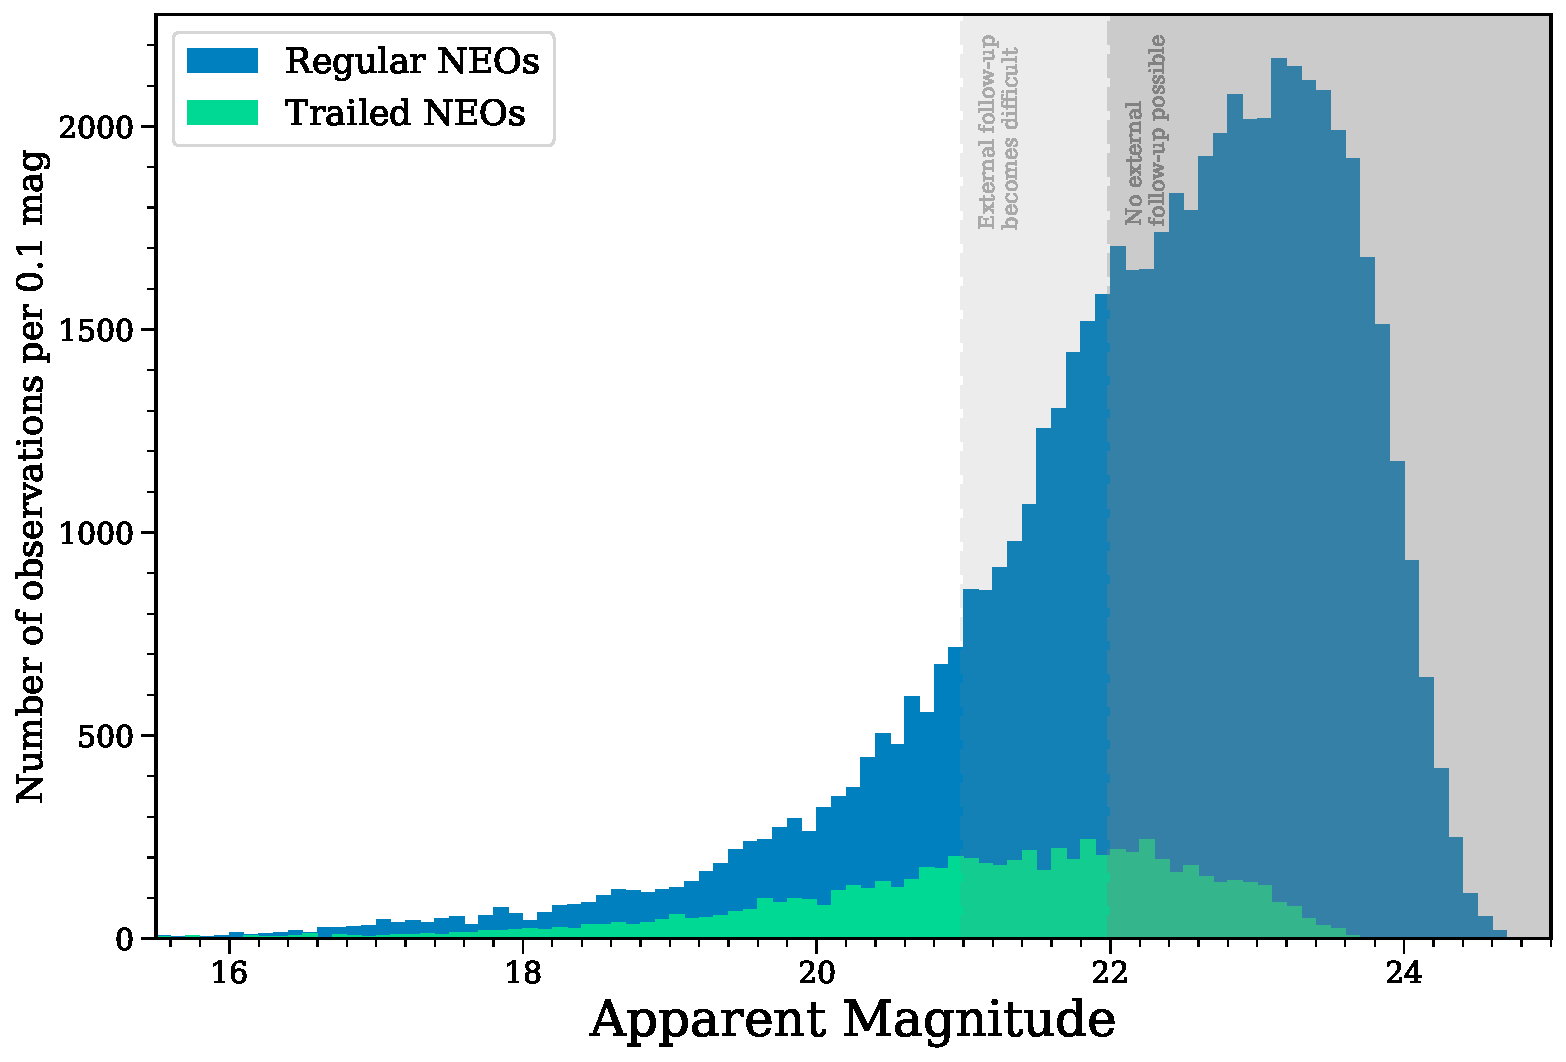
\includegraphics[width=\columnwidth]{figures/neo_magnitudes.pdf}
    \caption{Apparent magnitude of LSST NEO observations in year 1. Shaded regions indicate magnitudes at which external follow-up is difficult and impossible respectively.}
    \label{fig:neo_magnitudes}
\end{figure}

In Section~\ref{sec:digest2_score} we highlighted that many NEOs will be instantly recognised as such from their angular velocities. An object moving faster than 1.5 degrees per day will leave trails of 1.25 arcseconds in a 30s LSST exposure, corresponding to just over 6 pixels. We define any object surpassing this threshold as a trailed source. We find that approximately 10\% of NEOs observed by LSST will be trailed, whereas no MBA exceeds the necessary threshold. We predict that, on average, each night we would observe 21 trailed NEOs in tracklets with at least 2 observations.

In Figure~\ref{fig:neo_magnitudes} we show the distribution of apparent V-band magnitudes of NEOs in the first year of LSST. We find that only around 38\% of slower moving NEOs observed in the first year of LSST are bright enough for external follow-up (by our assumed threshold of $m < 22$). However, approximately 69\% of trailed NEOs are bright enough for external follow-up and so these may be a good target for the follow-up community in the first years of LSST.

\section{Summary \& Conclusions} \label{sec:conclusion}
We present new predictions for the NEOCP in the era of LSST. We performed mock LSST observations and used \dig{} to estimate the number of objects that LSST would send to the NEOCP using the current criteria. We created a new algorithm for predicting whether an object will be detected by LSST without external follow-up based on a single night of observations in order to reduce the load on the NEOCP. Our main conclusions can be summarised as:

\begin{enumerate}
    \item \textbf{Assuming no changes to listing criteria, the NEOCP will be overwhelmed by LSST submissions}: Once LSST observations begin, the traffic will increase by two orders of magnitude to around 1100 objects per night, whilst the purity would typically be 3\% but range as low as 0.2\% (Section~\ref{sec:traffic_basic}).
    \item \textbf{An algorithm to avoid the submission of objects likely re-observed by LSST itself improves the situation by a factor of $\mathbf{\sim4}$}: The algorithm we developed reduces the number of submitted candidates per night to approximately ${\sim}\npernightAlg{}$.
    \item \textbf{Reduction of the number of unknown MBAs should be prioritised in early years}: Even with avoidance of self-followed-up objects, the purity is still rather low (${\sim}\purityAlg{}\%$) due to the large MBA background (Section~\ref{sec:using_alg}).
    The major source of confusion with NEOs are previously unknown faint Main Belt asteroids. Therefore, when choosing between possible cadences (or selecting linking algorithms) we propose that those that maximize the early discovery of most MBAs are prioritized.
    \item \textbf{Early NEO follow-up strategies should be highly selective}\\Due to the vast number of unknown NEO-like MBA tracklets in the first year, the \dig{} score will perform poorly and NEO follow-up will be difficult. For the first year an ecliptic latitude cut can be used to remove MBAs from the sample. An additional cut in magnitude -- to prioritize bright and therefore large objects -- can further reduce the number of follow-up candidates. As the number of unknown MBAs reduces with time (thus increasing the purity of the NEO candidate sample), these constraints can be relaxed.
\end{enumerate}

The purpose of this paper was to bring these challenges into focus, and offer possible solutions. For example, in anticipation of LSST's start in early 2025, the types of algorithms and considerations we've developed here could be incorporated into tools such as NEOFixer \citep{NEOfixer}, the SNAPS broker \citep{SNAPS}, or other observation planning tools and aids. Also, the NEOCP inclusion criteria could be revisited and improved. One low-hanging fruit may be to consider updating the \dig{} score algorithm with the significantly improved knowledge of Solar System populations since \citet{Keys+2019} should be investigated.
\\

We end by stressing that these are {\em good} problems to have: they arise as the Rubin Observatory will dramatically enhance our ability to detect moving objects. This influx of observations will enable an unprecedentedly detailed census and understanding of NEOs as well as other populations of the Solar System.

\begin{acknowledgements}
    This material is based upon work supported in part by the National Science Foundation through Cooperative Agreement AST-1258333 and Cooperative Support Agreement AST-1202910 managed by the Association of Universities for Research in Astronomy (AURA), and the Department of Energy under Contract No. DE-AC02-76SF00515 with the SLAC National Accelerator Laboratory managed by Stanford University. Additional Rubin Observatory funding comes from private donations, grants to universities, and in-kind support from LSSTC Institutional Members.

    We thank Aren Heinze and Pedro Bernardenelli for insightful discussions in many aspects of this project. We thank Andy Connolly and Stephen Portillo for their advice in assessing the quality of the hybrid catalogue. We also thank Jessica Werk, Eric Agol, Željko Ivezić and Victoria Meadows for helpful feedback on an initial draft of this work.
    
    The authors further acknowledge the support from the University of Washington College of Arts and Sciences, Department of Astronomy, and the DiRAC Institute. The DiRAC Institute is supported through generous gifts from the Charles and Lisa Simonyi Fund for Arts and Sciences and the Washington Research Foundation. M. Juric wishes to acknowledge the support of the Washington Research Foundation Data Science Term Chair fund, and the University of Washington Provost’s Initiative in Data-Intensive Discovery.
    This work was facilitated through the use of advanced computational, storage, and networking infrastructure provided by the Hyak supercomputer system at the University of Washington.
\end{acknowledgements}

\software{\dig{} v0.19.2 \citep{Keys+2019}, \texttt{OpenOrb} \citep{Granvik+2009}, \texttt{difi} \citep{difi}, \texttt{THOR} \citep{Moeyens+2021}, \texttt{rubin\_sim} \citep{rubin_sim}, \texttt{Astropy} \citep{astropy:2013, astropy:2018, astropy:2022}, \texttt{astroML} \citep{VanderPlas+2012,astroMLText}, \texttt{Python} \citep{python}, \texttt{numpy} \citep{numpy}, \texttt{pandas} \citep{pandas_1.4.2, pandas_paper}, \texttt{matplotlib} \citep{matplotlib}, \texttt{scipy} \citep{Virtanen+2020}}

\bibliographystyle{aasjournal}
\bibliography{paper}{}

\restartappendixnumbering

\allowdisplaybreaks
\appendix

\section{Hybrid Catalogue Pipeline}\label{app:hybrid}
Many studies that make predictions for LSST use a synthetic catalogue of solar system objects that doesn't account for prior observations. In reality, we have already detected more than a million objects in the solar system and this number will continue to grow until LSST comes online. This means that, current predictions of detection rates will be inflated since a fraction of ``new'' detections may already be known. Therefore, for this paper we created ``hybrid'' catalogue that combines a synthetic catalogue with all known observations, whilst keeping the population distributions relatively unchanged.

We created the hybrid catalogue to be dynamic, such that we can run a single pipeline to merge in an updated version of \mpco{} as more objects are discovered in the time until LSST comes online. All code to reproduce this hybrid catalogue is open-source and available on GitHub\footnote{\url{https://github.com/dirac-institute/hybrid_sso_catalogue}}.

\subsection{Data preprocessing}
For the synthetic catalogue of the solar system we use \sss{}, the Pan-STARRS Synthetic Solar System Model \citep[\sss{}][]{Grav+2011}. We merge this synthetic catalogue with the latest version of \mpco{}\footnote{\url{https://minorplanetcenter.net//iau/MPCORB.html}}, a database of all currently known objects. We use \texttt{OpenOrb} \citep{Granvik+2009} to convert both catalogues to Cartesian coordinates and propagate all orbits until the same date.

\subsection{Merging algorithm}
The general idea for the merging algorithm is to inject each object from \mpco{} into \sss{}, replacing objects that are similar to those injected. An object's similarity is determined based on its position, $\va{x}$, velocity, $\va{v}$, and absolute magnitude (size), ${H}$.

We split each catalogue into bins of absolute magnitude linearly spaced from $-2$ to $28$ and perform the merge algorithm on each bin separately. For each bin we build a K-D trees for both catalogues based on the positions ($x, y, z$) of objects. For every \mpco{} object we query the \sss{} tree for the nearest $100$ objects up to a maximum distance of $0.1 \unit{au}$, excluding any that have already been matched to a different real object. From these remaining nearest neighbours, we select the \sss{} object with the closest velocity as the matched object. If there were no remaining neighbours, either because no synthetic objects were nearby or because all nearby objects had already been matched, then we directly add this real object without replacing a synthetic one.

To complete the merging process, we compile the matched object IDs and delete them from \sss{}. We then add the entirety of \mpco{} to the remaining catalogue, resulting in a hybrid catalogue.

\subsection{Assessing quality of hybrid catalogue}\label{app:hybrid_quality}
It is essential that the underlying distributions of the hybrid catalogue do not differ significantly from \sss{} so that we still accurately reproduce the solar system. In Figure~\ref{fig:hybrid_vs_s3m_dists}, we show the distributions of the absolute magnitude and six orbital elements in both the hybrid catalogue and \sss{}. It is evident that the distributions are essentially identical.

As a further check, we compared \mpco{} to the objects that were removed from \sss{}, since these should have nearly identical distributions other than MPCORB objects that had no matches. In Figure~\ref{fig:density_compare}, we show a comparison of the densities for the heliocentric $x$ and $y$ and it is clear that these distributions are left unchanged in the hybrid catalogue.
\begin{figure*}[htb]
    \centering
    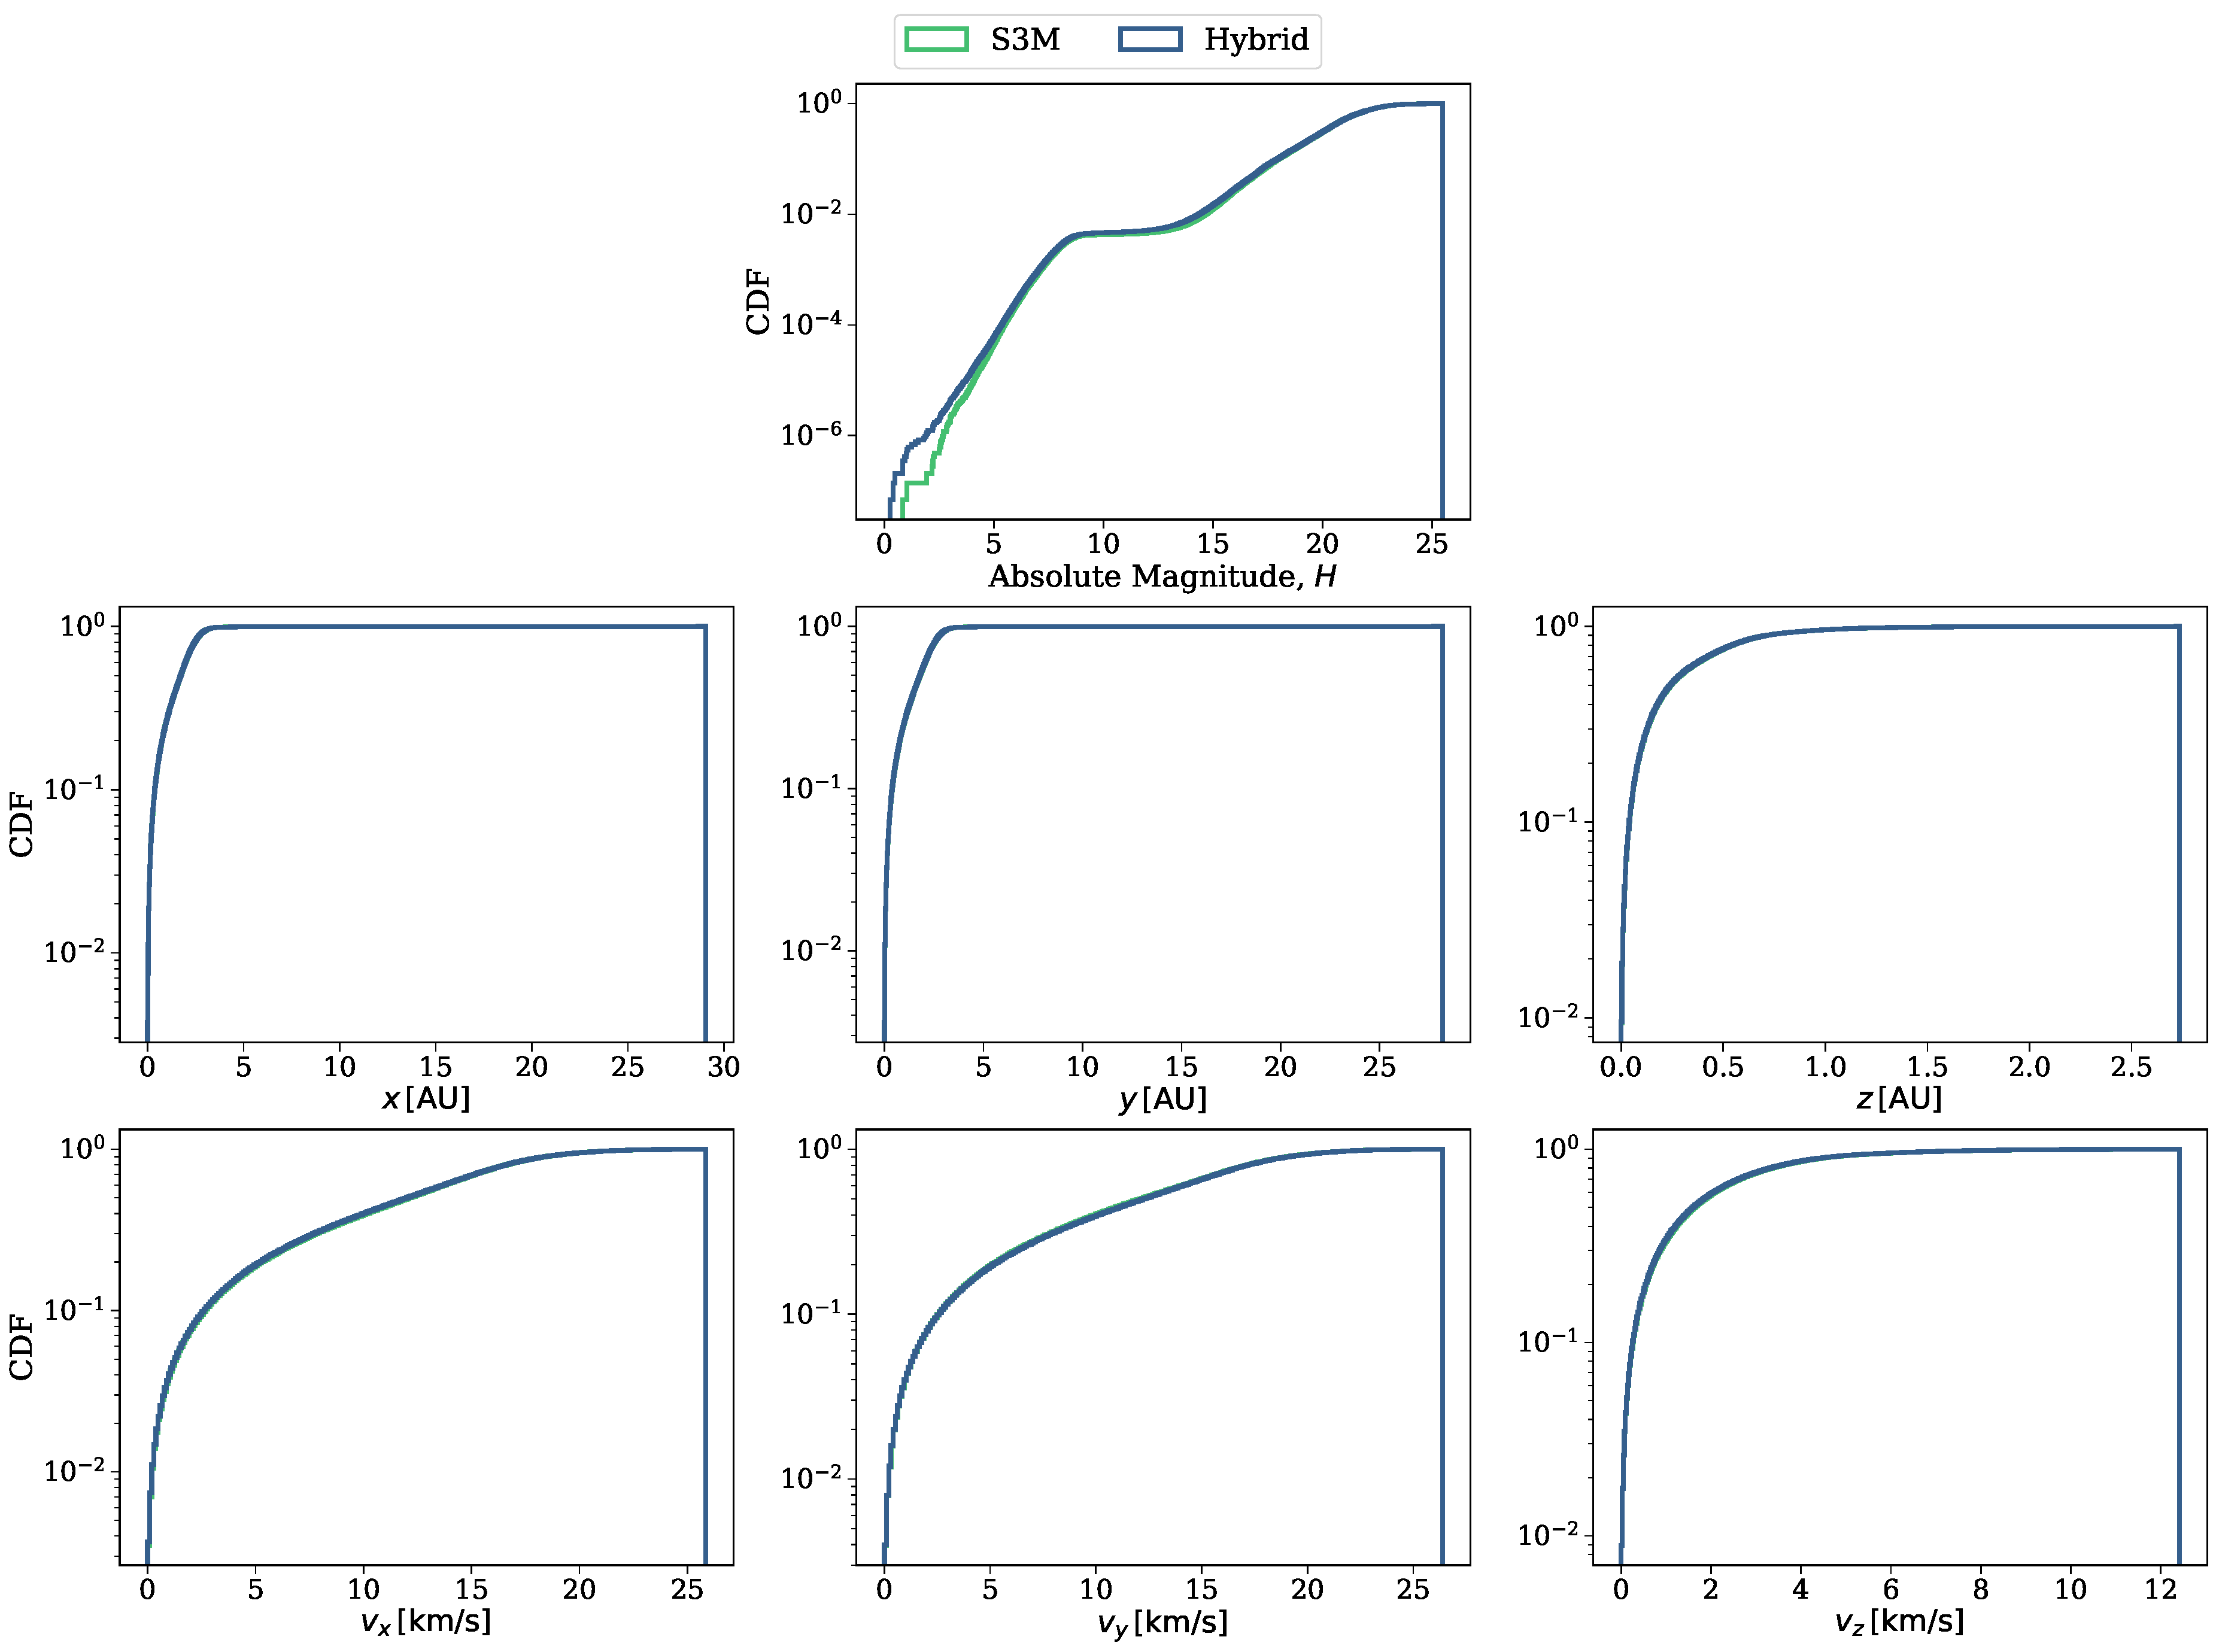
\includegraphics[width=\textwidth]{hybrid_vs_s3m_distributions.pdf}
    \caption{A comparison of the parameter distributions of \sss{} \citep{Grav+2011} and the hybrid catalogue we created.}
    \label{fig:hybrid_vs_s3m_dists}
\end{figure*}
\begin{figure}[htb]
    \centering
    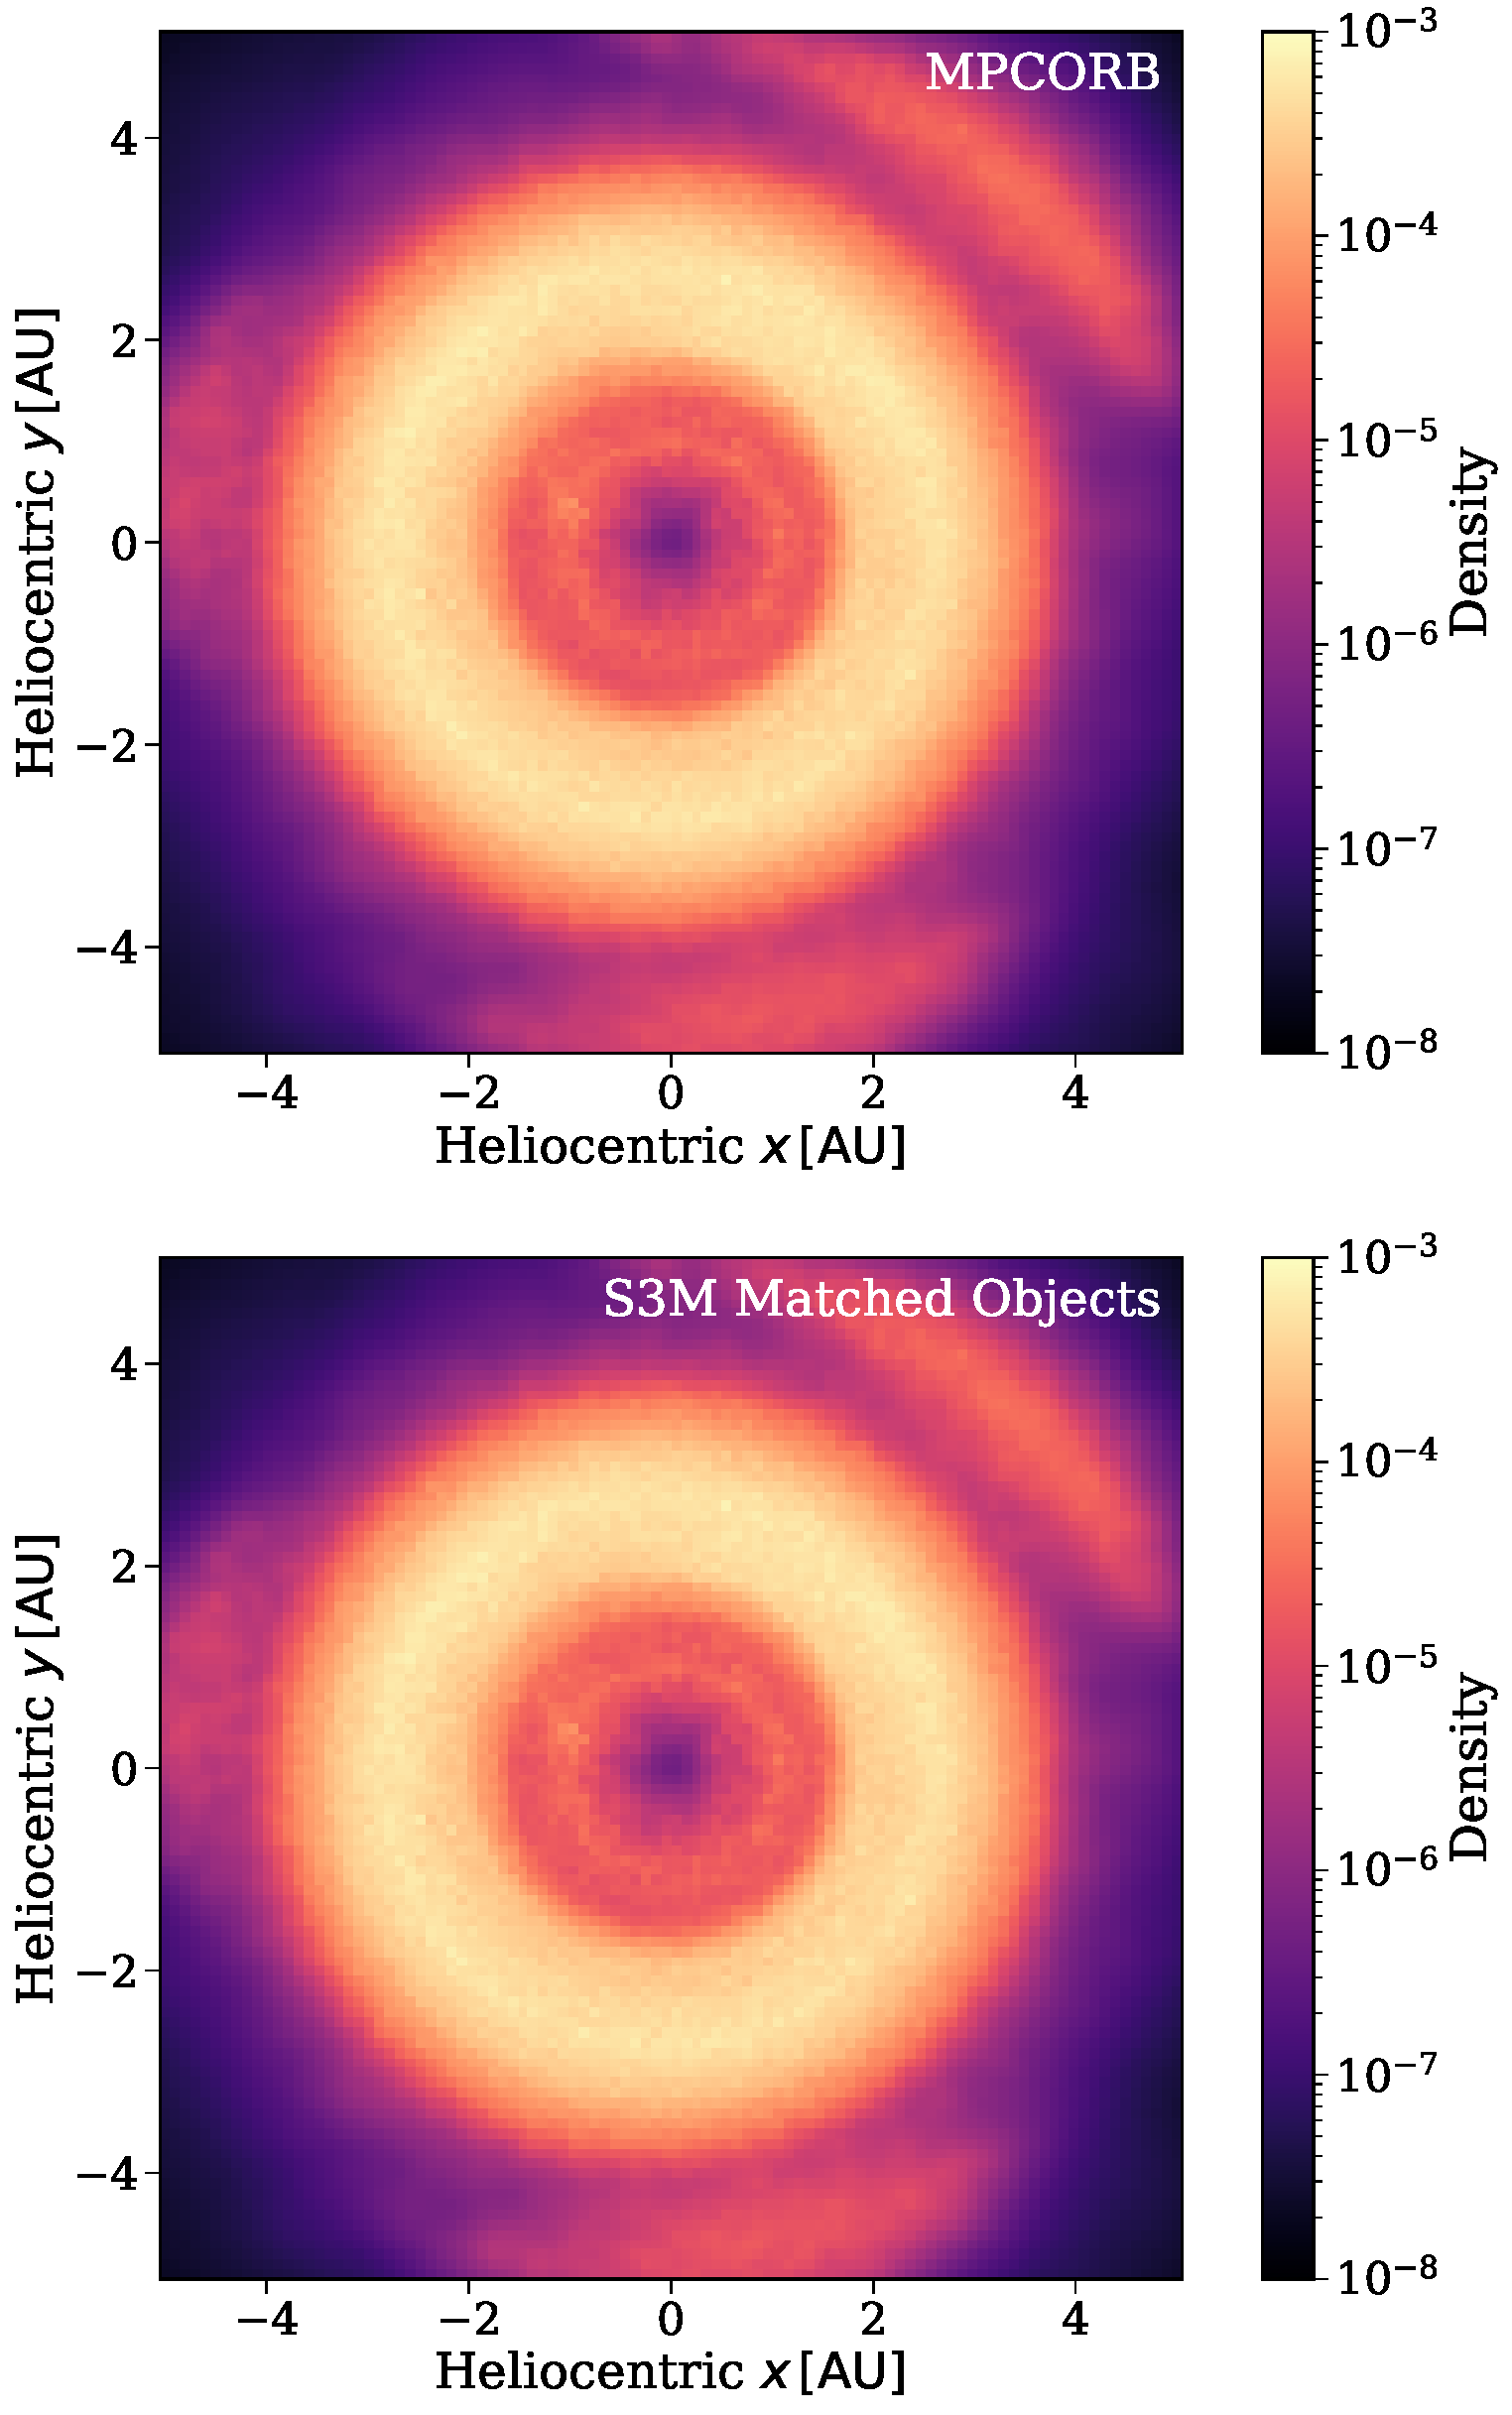
\includegraphics[width=0.48\textwidth]{density_comparisons.pdf}
    \raisebox{0.5\height}{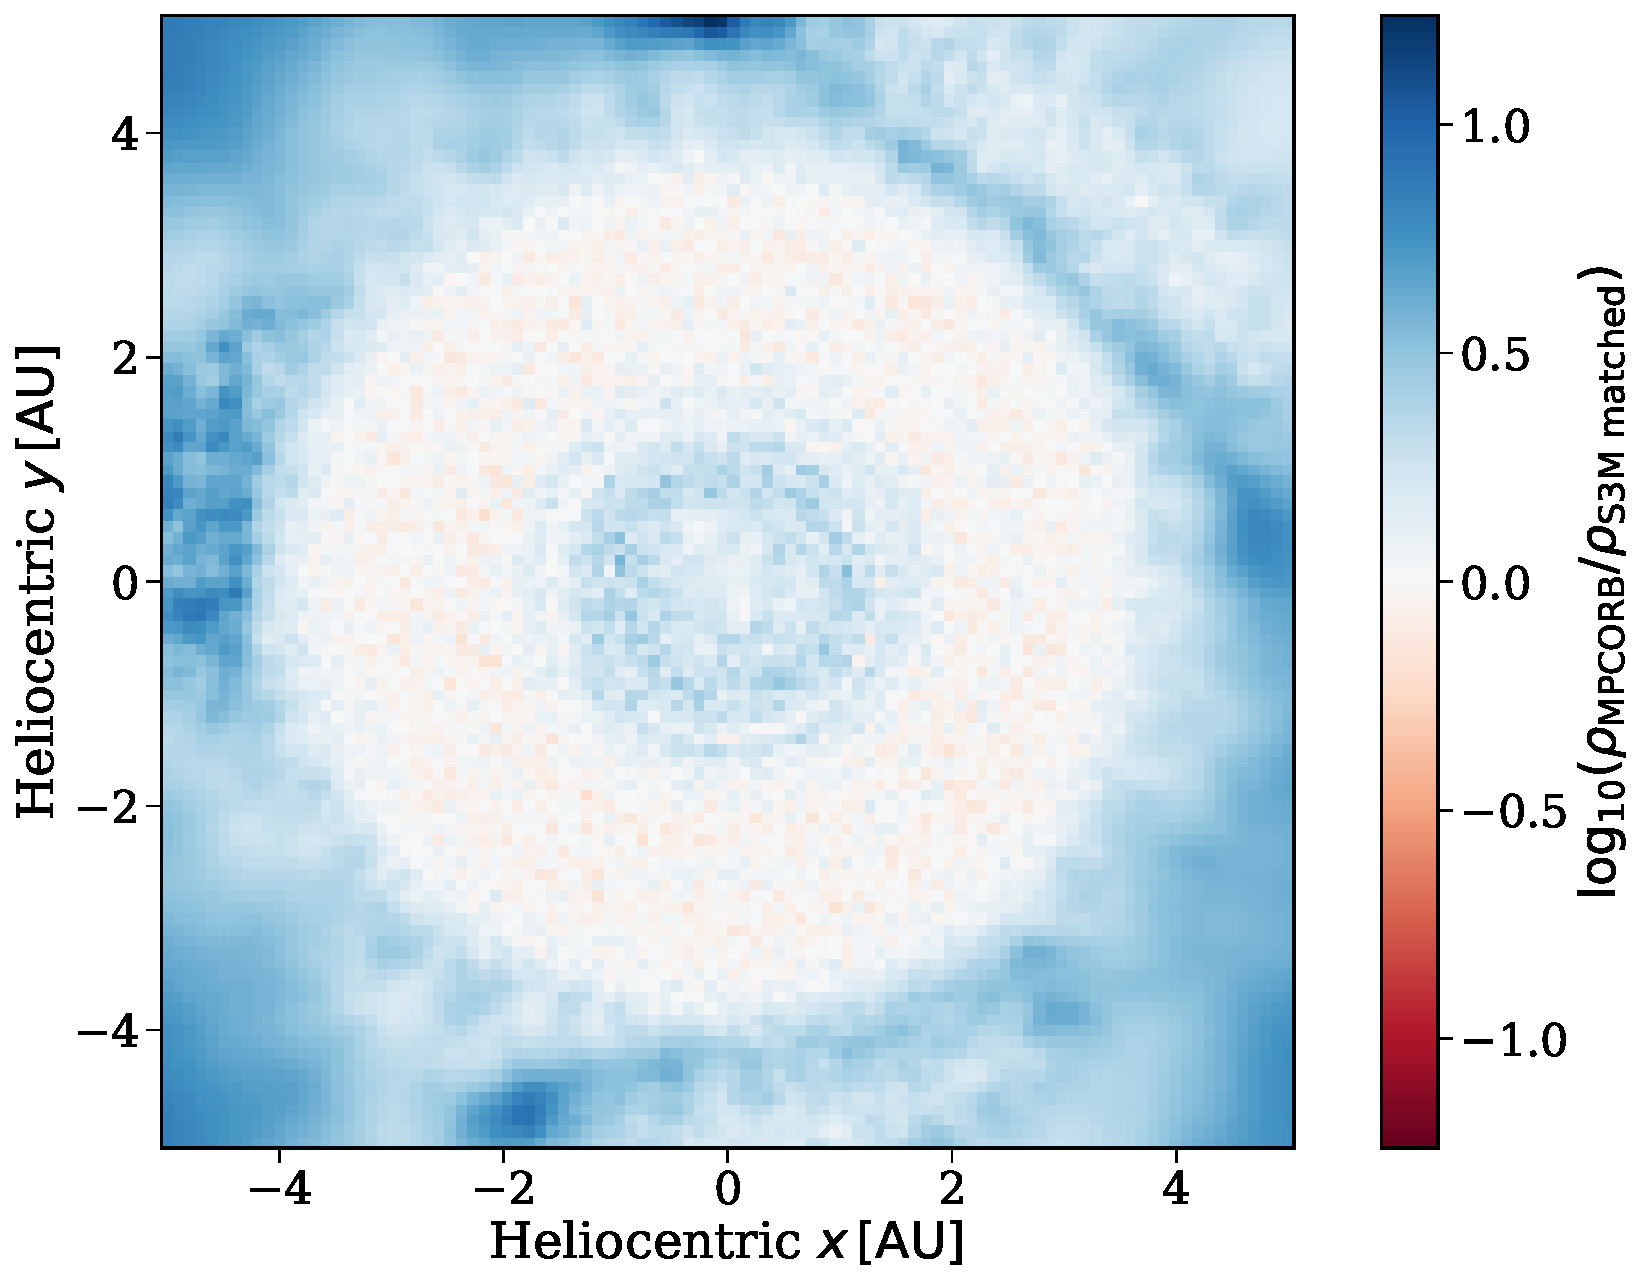
\includegraphics[width=0.48\textwidth]{density_residuals.pdf}}
    \caption{\textbf{Left:} A comparison of the density of \mpco{} objects with those objects that were matched in \sss{} by our hybrid catalogue pipeline. \textbf{Right:} Residuals between the two plots in the left panel.}
    \label{fig:density_compare}
\end{figure}

\end{document}